\documentclass[10pt,a4paper,titlepage,twoside]{report}
\usepackage{polski}
\usepackage[utf8]{inputenc}
\usepackage[T1]{fontenc}
\usepackage{graphicx}
\usepackage{sidecap}
\usepackage{wrapfig}
\usepackage{makecell}
\usepackage{subfig}
\usepackage{enumerate}
\usepackage{amssymb}
\usepackage{geometry}
\usepackage{pgfpict2e}
\usepackage{tikz}
\usepackage{wrapfig}
\usepackage{floatflt}
\usepackage{listings}
\usepackage{multirow}
\usepackage{comment}
\usepackage{array}
\usepackage{pbox}
\usepackage{setspace}
\usepackage{helvet}
\renewcommand{\familydefault}{\sfdefault}
\usepackage{chngcntr}
\usepackage{amsmath}
\usepackage[final]{pdfpages} 
\usepackage{xcolor,colortbl}
\usepackage{cite}
\counterwithin{figure}{chapter}
\newcommand{\done}{\cellcolor{teal}done}
\usepackage{xcolor}

\colorlet{punct}{red!60!black}
\definecolor{background}{HTML}{EEEEEE}
\definecolor{delim}{RGB}{20,105,176}
\colorlet{numb}{magenta!60!black}

\lstdefinelanguage{json}{
    basicstyle=\normalfont\ttfamily,
    numbers=left,
    numberstyle=\scriptsize,
    stepnumber=1,
    numbersep=8pt,
    showstringspaces=false,
    breaklines=true,
    frame=lines,
    backgroundcolor=\color{background},
    literate=
     *{0}{{{\color{numb}0}}}{1}
      {1}{{{\color{numb}1}}}{1}
      {2}{{{\color{numb}2}}}{1}
      {3}{{{\color{numb}3}}}{1}
      {4}{{{\color{numb}4}}}{1}
      {5}{{{\color{numb}5}}}{1}
      {6}{{{\color{numb}6}}}{1}
      {7}{{{\color{numb}7}}}{1}
      {8}{{{\color{numb}8}}}{1}
      {9}{{{\color{numb}9}}}{1}
      {:}{{{\color{punct}{:}}}}{1}
      {,}{{{\color{punct}{,}}}}{1}
      {\{}{{{\color{delim}{\{}}}}{1}
      {\}}{{{\color{delim}{\}}}}}{1}
      {[}{{{\color{delim}{[}}}}{1}
      {]}{{{\color{delim}{]}}}}{1},
}

\begin{document}

%
\includepdf[pages=1-4]{header.pdf}

\includepdf[pages=1-2]{formal-header.pdf}

\newgeometry{tmargin=2.5cm, bmargin=2.5cm, lmargin=3.5cm, rmargin=2.5cm}
\setlength{\parindent}{1.25cm}


\newgeometry{top=2.5cm, bottom=2.5cm, left=3.5cm, right=2.5cm}
\setcounter{page}{3}
\onehalfspacing
\justify
\section*{Streszczenie}
\addcontentsline{toc}{section}{Streszczenie}
\indent\indent Prawdą jest, że dzisiejsze społeczeństwo informacyjne rozwija się niesamowicie szybko. Człowiek we współczesnym świecie pragnie coraz większego rozwoju i unowocześnień technologicznych. Niestety napotyka na ograniczenia w dziedzinach fizyki i chemii,które sprawiają,że coraz trudniej będzie wytwarzać szybsze procesory opierając się na klasycznych metodach. Administratorzy i właściciele centrów danych nie mogą wymieniać procesorów na szybsze, co powoduje konieczność kupowania kolejnych fizycznych serwerów. Również czynniki takie jak bezpieczeństwo, redundancja danych czy zapewnienie odpowiednio wysokiego poziomu świadczenia usług zmuszają do rozbudowy infrastruktury i kupowania kolejnych serwerów. Doprowadza to do zwiększenia kosztów utrzymania centrum danych czy do bardziej skomplikowanego procesu serwisowania.Te właśnie czynniki generują potrzebę zaprojektowanie mechanizmów pozwalających efektywnie wykorzystywać istniejące centra danych

 Christos Kozyrakis, doktor z Uniwersytetu Stanforda w jednej ze swoich prac omawia problem niskiej utylizacji centrum danych. By poprawić tą sytuację należało by umieszczać wiele niezależnych od siebie zadań na tych samych komputerach by efektywniej wykorzystywać dostępne na nich zasoby. Wymaga to opracowania wydajnych mechanizmów izolacji oraz optymalnych zasad rozdzielania zadań pomiędzy dostępne zasoby. Dzięki odpowiednio zaprojektowanym mechanizmom izolacji zadania nie będą ryzwalizowały o zasoby, zaś wykonywane operacje będą wykonywane niezależnie od innych procesów. Przy takim założeniu nawet awarie i błędy w innych zadaniach nie powinny interferować pozostałych. Dodatkowo zadania na klastrze powinny być tak rozdzielone by w pełni optymalizować obecne na nim zasoby. Na przykład zadania korzystające z tych samych portów powinny być uruchomione na innych komputerach. Wskazanym też jest uruchamianie na tym samym komputerze zadań obliczeniowych (mocno zużywających procesor) oraz zadań wykorzystujących przestrzeń dyskową (na przykład instancje klastrowalnych baz danych).

Głównym celem tej pracy jest analiza obecnych na rynku rozwiązań związanych z konteneryzacją aplikacji. Jest to bardzo młode pojęcie a pierwsze produkty ją wykorzystujące są ciągle rozwijane i często zmieniają się architektonicznie. W tej pracy dokonam testów izolacji poszczególnych rozwiązań. Drugim ważnym elementem mojej pracy jest analiza orkiestratorów zadań uruchamianych w kontenerach. Skupię się tutaj na rozwiązaniu Mesos oraz systemach szeregowania zadań, które mogą z nim współpracować. 
\newline
\newline
\newline
\noindent \textbf{Słowa kluczowe:} chmury obliczeniowe, centrum danych, konteneryzacja, izolacja, orkiestracja

\newpage
\section*{Abstract}
\addcontentsline{toc}{section}{Abstract}

\indent\indent Incredibly rapid development of the information society and technological development has made it necessary to design mechanisms to effectively utilize existing data centers. Due to the limitations of physics and chemistry, it is more difficult to produce faster processors based on classical methods. Administrators and data center owners cannot swap CPUs to faster, which results is the need to purchase more physical servers. Also, factors such as security, data redundancy, or providing a high level of performance are forcing the infrastructure to go down and buying more servers. This leads to increased data center maintenance costs and to a more complex servicing process.

 Christos Kozyrakis,Stanford University Phd. discusses the problem of low data center utilization in one of his papers. In order to improve this situation, administrator should to place many independent tasks on the same computers to make more efficient use of available resources. This requires the development of efficient isolation mechanisms and optimal separation of tasks between available resources. Due to the well-designed isolation mechanisms, tasks will not rationalize resources, and operations will be performed independently of other processes. Even failures and errors in other tasks should not interfere with the rest. In addition, tasks on the cluster should be separated so as to fully optimize the resources on the cluster. For example, tasks that use the same ports should run on other computers. It is also advisable to run computational tasks (heavy CPU usage) and disk space tasks (for example instances of clustered databases) on the same computer.

The main purpose of this paper is to analyze the current market solutions related to containerized applications. Containerization is a very young concept and the first uses of it are constantly evolving and often changing architecturally. In this work I will test isolation of individual solutions. The second important element of this work is the analysis of the task force operators in containers. I will focus here on the Mesos solution and task scheduling systems that can work with it.
\newline
\newline
\newline
\textbf{Keywords:} cloud computing, data center, containerization, izolation, orchestration

\newpage
\newgeometry{top=2.5cm, bottom=2.5cm, left=2.5cm, right=3.5cm}

\tableofcontents


\newpage
\newgeometry{top=2.5cm, bottom=2.5cm, left=2.5cm, right=3.5cm}
\section*{Wykaz ważniejszych oznaczeń i skrótów}
\addcontentsline{toc}{section}{Wykaz ważniejszych oznaczeń i skrótów}

API - (ang. \textit{Application Programming Interface}) interfejs programowy aplikacji \\ \newline
CLI - (ang. \textit{Command Line Interface}) interfejs wiersza poleceń \\ \newline
DC - (ang. \textit{Data Center}) Centrum Danych \\ \newline
DC/OS - (ang. \textit{Data Center Operation System}) komercyjna wersja systemu Mesos \\ \newline
ELK - (ang. \textit{ElasticSearch Logstash Kibana}) zestaw narzędzi, które uruchomione jednocześnie umożliwiają łatwe monitorowanie i przeszukiwanie logów klastra. \\ \newline
HTTP - (ang. \textit{Hypertext Transfer Protocol}) interfejs programowy aplikacji \\ \newline
IP - (ang. \textit{IP address}) adres IP \\ \newline
LDAP - (ang. \textit{Lightweight Directory Access Protocol}) lekki protokół usługi katalogowej \\ \newline
NIS - (ang. \textit{Network Information Service}) serwis informacji sieciowej \\ \newline
NVMe - (ang. \textit{Non-Volatile Memory Host Controller}) kontroler pamięci nieulotnych \\ \newline
OCI - (ang. \textit{Open Container Initiative}) inicjatywa otwartych kontenerów - projekt Fundacji Linux \\ \newline
SATA - (ang. \textit{Serial Advanced Technology Attachment}) szeregowa magistrala komputerowa \\ \newline
SQL - (ang. \textit{Structured Query Language}) strukturalny język zapytań \\ \newline
RAM - (ang. \textit{Random access memory}) pamięć o dostępie swobodnym \\ \newline
UI - (ang. \textit{user interface}) interfejs użytkownika \\ \newline
URL - (ang. \textit{Uniform Resource Locator}) ujednolicony format lokacji zasobów \\ \newline

\newpage
\newgeometry{top=2.5cm, bottom=2.5cm, left=2.5cm, right=3.5cm}
\onehalfspacing

\chapter{Wstęp i cel pracy}
\section{Charakterystyka klastrów obliczeniowych}
\indent \indent Na przestrzeni lat znacząco wzrosła liczba użytkowników Internetu\cite{ad1}. Obecnie utrzymywanie kilku stron internetowych, odwiedzanych każdego dnia przez wielu użytkowników jest znacznie trudniejsze niż kiedyś\cite{ad1}. Liczba treści w Internecie sprawia, że bazy danych rosną w zastraszającym tempie, a bardziej skomplikowane zapytania konsumują duże ilości zasobów na maszynach. Aby walczyć z tymi problemami można optymalizować kod, zwiększać liczbę dostępnych zasobów - dokładać pamięci operacyjnej, stosować szybsze dyski czy używać procesorów z większą ilością rdzeni, lub wyższym taktowaniem. Mimo takich działań administratorzy serwerów niebawem znajdą się w sytuacji, w której konieczne będzie użycie kolejnej maszyny, aby poradzić sobie z obsługą generowanego przez użytkowników ruchu \cite{ad2}. Stworzy to wiele problemów z którymi administrator będzie musiał sobie poradzić: współdzielenie oraz synchronizowanie bazy danych między maszynami, rozkładanie obciążenia między maszyny i wiele innych \cite{ad2}.

Jeśli strona internetowa osiągnie prawdziwy sukces i obsługa będzie wymagała kolejnych serwerów, administrator zetknie się z problemem monitorowania maszyn, wydzielenia dysków czy tworzeniem kopii zapasowych. Wiele serwerów to też problem utylizacji zasobów. Konieczne jest takie rozłożenie zadań na naszym klastrze, by zmaksymalizować użycie zasobów na poszczególnych serwerach - każda nieużywana pamięć to strata pieniędzy i energii\cite{ad3}.

\begin{figure}[ht!]
	\centering
	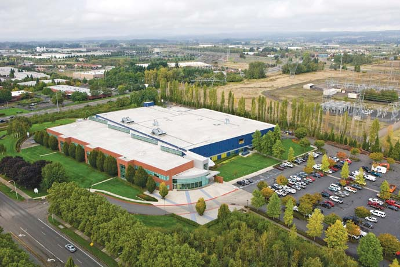
\includegraphics[scale=0.7]{pics/Selection_615.png}
	\caption{Centrum danych Facebooka w Oregonie.}
	\label{facebook_dc}
\end{figure}


Dla przykładu firma Facebook, na samym początku swojego istnienia obsługiwała cały ruch za pomocą wyłącznie jednej maszyny\cite{ad4}. Było to w czasach gdy serwis ten nie wspierał jeszcze publikowania obrazków, czy filmów przez użytkowników. W kwietniu 2008 roku centrum danych Facebooka liczyło już 10 tysięcy maszyn, by dwa lata później osiągnąć już 60 tysięcy. Obecnie korporacja nie zdradza informacji ile serwerów utrzymuje, ale rozmiar ich farmy serwerów w Oregonie (rys. \ref{facebook_dc}), mówi sam za siebie - 307 tysięcy metrów kwadratowych\cite{ad5}.

Powyższy problem dotyczy tylko jednego typu zadania, czyli hostingu wymagającego web serwisu. Współczesny świat współtworzony jest przez wiele rodzajów zadań: konwersja wideo, obliczanie skomplikowanych matematycznych równań, przechowywanie i prezentowanie map i wiele innych. Poszczególne rodzaje zadań często interferują ze sobą. Ich umieszczanie na jednym serwerze może doprowadzić do walki o zasoby między procesami. Pojawia się więc problemem utylizacji serwerowni, czyli rozłożenia zadań tak by nie kolidowały ze sobą, ale także aby zminimalizować ilość nieużywanych zasobów\cite{ad5}.

\subsection{Podział klastrów obliczeniowych}\indent \indent Ze względu na pełnione funkcje, możemy wyróżnić następujące rodzaje klastrów obliczeniowych\cite{ad6}.

\begin{itemize}
	\item \textbf{Klastry wydajnościowe (ang. \textit{High Performance Computing Clusters})} - moc obliczeniowa jest wykorzystywana do przeprowadzania bardzo skomplikowanych obliczeń matematycznych, trwających nawet wiele miesięcy. Służą do przetwarzania jednego rodzaju danych (np. porównywanie kodów DNA, przygotowywanie markerów rakowych itp.).
	\item \textbf{Klastry równoważące obciążenie (ang. \textit{Load Balancing Clusters})} - ich główne zadanie polega na równoważnym dystrybuowaniu obciążenia między poszczególne serwery  (węzły klastra). Tego typu klaster instaluje się w systemach, w których bardzo istotny jest czas reakcji na zadanie klienta. \textit{Load balancer} przesyła nadchodzące żądania obsługi do węzłów, które posiadają niezagospodarowane w danej chwili moce obliczeniowe, odciążając tym samym węzły, które są w danym momencie mocno obciążone i zbyt wolno odpowiadają by obsłużyć kierowane od klienta żądanie. Przykładowe zastosowanie takiego klastra to hosting stron internetowych, czyli udostępnianie mniej lub bardziej złożonych aplikacji internetowych klientowi końcowemu. Często wymaga to zainstalowania na klastrze systemów bazodanowych oraz interpreterów specyficznych dla technologii w której wytworzony jest web serwis.
	\item \textbf{Klastry niezawodnościowe (ang. \textit{High Availability Clusters})} - klastry o wysokiej dostępności. Klastry tego typu nie zwiększają wydajności serwisów, a mają jedynie eliminować tzw. pojedynczy punkt awarii (ang. Single Point of Failure) - w razie uszkodzenia jednego z serwerów jego zadania są, w sposób niewidoczny dla użytkowników, przejmowane przez inny węzeł klastra.
\end{itemize}

\subsection{Podział chmur ze względu na zainstalowane oprogramowanie}\indent \indent Klaster obliczeniowych na którym zainstalowano i skonfigurowano odpowiednie oprogramowanie będziemy nazywać chmurą obliczeniową. W zależności od zainstalowanego na klastrze oprogramowania, możemy wyróżnić następujące rodzaje chmur\cite{ad6}:
\begin{itemize}
	\item \textbf{Infrastructure as a Service (IaaS)} - zasoby serwerów klastra są wydzielane i odizolowywane od siebie a następnie przedstawiane są użytkownikowi końcowemu jako niezależne serwery. Ten rodzaj chmur obliczeniowych mogą wykorzystywać firmy, które chcą sprzedawać niewielkie serwery swoim klientom. Model tej usługi polega na dostarczaniu klientowi infrastruktury informatycznej czyli sprzętu, oprogramowania oraz serwisowania. Klient wykupuje na przykład konkretną liczbę serwerów, przestrzeni dyskowej, lub określony zasób pamięci i mocy obliczeniowej. Nie oznacza to jednak, że sprzęt fizycznie zostanie zainstalowany w siedzibie klienta\cite{ad7}. W tym modelu zdarza się, że klient dostarcza usługodawcy własne oprogramowanie do zainstalowania na wynajmowanym sprzęcie.
	\item \textbf{Platform as a Service (PaaS)} - w tym modelu sprzedaje się gotowe, często dostosowany do potrzeb użytkownika, komplet aplikacji. Nie wiąże się to z koniecznością zakupu sprzętu ani instalacją oprogramowania. Wszystkie potrzebne programy znajdują się na serwerach dostawcy \cite{ad9}. Klient po swojej stronie ma dostęp do interfejsu (na ogół w postaci ujednoliconego środowiska pracy) poprzez program (klienta) np. przeglądarkę internetową. W tym modelu usługi najczęściej dostępne są dla użytkownika z dowolnego połączonego z Internetem komputera.
	\item \textbf{Software as a Service (SaaS)} - aplikacja jest przechowywana i wykonywana na komputerach dostawcy usługi i jest udostępniana użytkownikom przez Internet. Eliminuje to potrzebę instalacji i uruchamiania programu na komputerze klienta. W tym modelu użytkownik oddaje kontrolę ddostawcy i obowiązek zapewnienia ciągłości jego działania spoczywa na nim. Istotą biznesową oprogramowania w modelu SaaS, decydującą o jej rosnącej popularności jest to, że użytkownik kupuje działające rozwiązanie o określonej funkcjonalności bez konieczności wchodzenia w zagadnienia związane z infrastrukturą informatyczną oraz zapleczem technicznym. W wielu przypadkach SaaS umożliwia dostęp do najnowszych technologii informatycznych bez długotrwałych wdrożeń i dużych inwestycji \cite{ad8}.
	\item \textbf{Data as a Service (DaaS)} - polega na udostępnieniu użytkownikowi przestrzeni dyskowej, którą może wykorzystać do przechowania plików \cite{ad10}, np. zdjęć, muzyki, filmów itd. Chmury tego typu oferują interfejs (np. w postaci web serwisu), który umożliwia łatwą komunikację i zarządzanie utrzymywanymi plikami. Interfejsy w takiej chmurze pozwalają na łatwe dzielenie się danymi z innymi użytkownikami, np. przy pomocy odpowiednich linków.
	\item \textbf{Storage as a Service (STaaS)} - polega na udostępnieniu użytkownikowi przestrzeni dyskowej, która może być przez niego dowolnie wykorzystana. W tym modelu klient końcowy otrzymuje bezpośredni dostęp do urządzeń lub bloków pamięci i to po jego stronie leży zaprojektowanie mechanizmu, który będzie z tych udostępnionych zasobów korzystał\cite{ad10}. Jest to główna różnica między chmurą typu DaaS, w której to użytkownik ma przygotowany interfejs, również uruchomiony w chmurze.
	\item \textbf{Security as a Service (SecaaS)} - podejście polegające na uruchamianiu oprogramowania antywirusowego w chmurze. Klient takiej chmury otrzymuje wszystkie funkcje programów antywirusowych (skanowanie plików, heurystyka itd.) bez konieczności uruchamiania antywirusa na swoim sprzęcie. Ze względu na ogromne ilości danych przesyłanych między chmurą z antywirusem, a końcowym użytkownikiem, tego typu rozwiązania mogą mieć głównie zastosowania w lokalnych serwerowniach (wysokie przepustowości między maszynami w jednym centrum danych).
\end{itemize}
\subsection{Podział chmur ze względu na lokalizację infrastruktury technicznej}
\begin{itemize}
	\item \textbf{Chmura prywatna (ang. \textit{Private Cloud})} - rozwiązanie polega na zakupieniu przez dany ośrodek fizycznych serwerów, podłączeniem ich w serwerowni oraz zainstalowaniem całego oprogramowania od zera \cite{ad10}. Chmura prywatna to inwestycja, która wymaga dużego wkładu początkowego (zakup serwerów), oraz ponoszenia ciągłych kosztów związanych z zasilaniem i chłodzeniem uruchomionych serwerów. Nie bez znaczenia pozostaje koszt związany z zatrudnieniem kadry i administratorów odpowiedzialnych za utrzymanie serwerów jak i całego centrum danych. Chmura prywatna daje użytkownikowi końcowemu pełną swobodę i możliwość całkowitego ingerowania w swoją infrastrukturę. Odpowiednio przygotowana polityka bezpieczeństwa będzie dawała pewność, że nikt postronny nie ma dostępu do danych. Własna serwerownia to też wyższe prędkości i uniezależnienie się od powolnie działającej sieci Internet \cite{ad11}.
	\item \textbf{Chmura publiczna (ang. \textit{Public Cloud})} - rozwiązanie polega na wykupieniu u wybranego dostawcy (ang. providera) odpowiedniego rozwiązania. W tym podejściu cała infrastruktura z której korzystamy znajduje się u dostawcy, zaś klient otrzymuje do niej dostęp poprzez sieć Internet i odpowiednie protokoły dostępu \cite{ad12}. W rozwiązaniach typu Public Cloud wszystkie dane są trzymane na infrastrukturze dostawcy, a co za tym idzie klient chmury nie ma nad nimi pełnej kontroli. Jest to jeden z głównych powodów, dla których firmy szczególnie chroniące swoje dane, bądź pracujące nad rozwiązaniami poufnymi niechętnie korzystają z tego rozwiązania \cite{ad11}. Na rynku chmur obliczeniowych trwa niekończąca się dyskusja \cite{ad13}, na temat opłacalności chmur publicznych w stosunku do prywatnych. Używanie chmury publicznej generuje koszty, które ponoszone są przez regularnie przez klienta (comiesięczne rachunki). Chmury publiczne dostosowują się do obciążenia i wymagań użytkownika, tzn. jeśli dotychczasowe zasoby są niewystarczające by obsłużyć ruch, zasoby klienta są automatycznie powiększane z jednoczesnym podwyższeniem kwoty do zapłacenia w kolejnym okresie rozliczeniowym. W ostatecznym rozrachunku, po kilku latach używania i opłacania chmury publicznej może się okazać, że całkowite wydatki znacznie przewyższyły jednorazowy wydatek, który trzeba by ponieść by zakupić na własny użytek chmurę prywatną. Warto w tym miejscu wspomnieć o ważnej zalecie chmury publicznej, tj. możliwość kolokacji zasobów i federowania uruchomionych usług. Dostawcy chmur publicznych często posiadają wiele centrów danych \cite{ad11}. Zwiększa to bezpieczeństwo danych – nawet atak na jakiś kraj i całkowity jego paraliż nie spowoduje wyłączenia naszych usług, gdyż będzie możliwe ich natychmiastowe uruchomienie w centrum danych po drugiej stronie globu. Takie rozwiązanie umożliwia również odpowiednie dzielenie obciążenia naszych usług o ile tylko są one do tego przystosowane. Użytkownicy końcowi usługi w chmurze, łączący się np. z USA skorzystają z centrów danych rozlokowanych w Ameryce Północnej, zaś klient z Europy połączy się z odpowiednim dla niego centrum danych ze starego kontynentu \cite{ad11}.
	\item \textbf{Chmury hybrydowe (ang. \textit{Hybrid Cloud})} - rozwiązanie polegające na połączeniu chmur publicznych i chmur prywatnych \cite{ad13}. Celem budowy takiej chmury jest uwypuklenie zalet obu rozwiązań, tj. przechowywanie danych w chmurze prywatnej, zaś dokonywanie obliczeń, bądź serwowanie treści web serwisu po stronie chmury publicznej. Innym często spotykanym rozwiązaniem jest uruchamianie zadań w chmurze prywatnej, zaś chmura publiczna jest używana do przechowywania kopii bezpieczeństwa \cite{ad13}.
\end{itemize}

\subsection{Podział klastrów obliczeniowych}\indent \indent Uruchamianie aplikacji na chmurach obliczeniowych stwarza wiele problemów, które nie były spotkane przy klasycznym podejściu \cite{ad14}. Mowa tu między innymi o:
\begin{itemize}
	\item Napisaniu aplikacji w taki sposób by działała na chmurze.
	\item Aplikacja powinna współpracować z innymi uruchomionymi instancjami.
	\item Odpowiednim odizolowaniu od siebie zadań na poszczególnych serwerach.
	\item Optymalnym podzieleniu zadań pomiędzy dostępne zasoby.
	\item Zaprojektowaniu architektury sieciowej w serwerowni, tak aby była odporna na ataki z zewnątrz oraz możliwie optymalizowała ruch pomiędzy maszynami.
	\item Osiągnięciu wysokiego poziomu utylizacji całego centrum danych.
\end{itemize}

\section{Cel oraz zakres projektu}
\indent \indent Projekt realizowany jest w ramach pracy dyplomowo-magisterskiej na semestrze trzecim studiów stacjonarnych II stopnia na kierunku “Informatyka” wydziału Elektroniki, Informatykii Telekomunikacji Politechniki Gdańskiej.

W poprzednim podrozdziale wypisałem kilka podstawowych problemów dotyczących chmur obliczeniowych. W niniejszej pracy chciałbym szczególnie skupić się na jednym z nich, mianowicie utylizacji centrum danych. Wykładowca z uniwersytetu Stanford, Christos Kozyrakis w jednej ze swoich publikacji \cite{ad3} udowadnia tezę, która mówi o bardzo niskim poziomie utylizacji całego centrum danych. Według jego dowodów poziom utylizacji w typowym centrum danych to około 20 procent. Doktor Kozyrakis wskazuje, jak drogie jest utrzymywanie centrum danych (chłodzenie, zasilanie) w stosunku do poziomu utylizacji jaką właściciel serwerowni jest w stanie utrzymać. W pracy wspiera się pogląd, że zamiast inwestować w kolejne serwery, wcześniej należy podjąć próby zoptymalizowania pracy całego centrum danych. Według autora dokumentu, należy przyjrzeć się dwóm kwestiom: odpowiedniego odizolowania zadań (tak aby nie interferowały one między sobą) oraz optymalnego i odpowiedzialnego rozdzielenia je na poszczególne fizyczne serwery, którymi dysponuje administrator.

Moja praca magisterska dotyczy analizy narzędzia Mesos i jego \textit{frameworków}, pod kątem zarządzania zasobami w centrum danych, ze szczególnym zwróceniem uwagi na zwiększanie poziomu utylizacji całej serwerowni. W pracy dokonam przeglądu kilku istniejących na rynku \textit{frameworków} i przeprowadzę krótką analizę w oparciu o dokonane w ramach projektu magisterskiego pomiary. Krótko opiszę i zbadam kilka mechanizmów izolacji wykorzystywanych obecnie.

Rozwiązanie Mesos wybrałem ze względu na jego stabilność i wysoki poziom adopcji na rynku chmur obliczeniowych. Mesos’a wykorzystuje wiele firm \cite{ad16}, np.: Allegro, Twitter, eBay czy Samsung. Na rynku dostępnych jest jednak więcej narzędzi. Więcej informacji na ich temat opiszę w dalszej części pracy.

Całe oprogramowanie, które zostało przeanalizowane bądź opisane w tej pracy było oprogramowaniem otwartym i darmowym. Również wszystkie produkty powstałe wraz z tą pracą są udostępnione na takiej właśnie licencji.

Mesos jest rozwiązaniem rozpowszechnianym na licencji Apache 2.0. Od lat produktem zajmuje się firma Mesosphere. Firma ta przygotowała grupę rozwiązań związanych z chmurami obliczeniowymi oraz silnie włączyła się w rozwijanie Mesosa. Dzięki wsparciu tej firmy udało się wydać wersję 1.0 (przeskok z wersji 0.26). Przyłączenie się Mesosphery do rozwoju Mesosa przyniosło też minusy. Najbardziej znaczącym z nich jest spadek zainteresowania „czystym” Mesosem na rzecz produktu Mesosphery „DC/OS” – Data Center Operating System. Narzędzie prócz samego Mesosa zawiera zaawansowany instalator, wsparcie dla sklastrowanego systemu przechowywania danych, zunifikowany dostęp do logów oraz rozbudowanego klienta CLI. Rozwiązanie DC/OS dostępne jest w dwóch wersjach - darmowej oraz skierowanej do klientów biznesowych. Wykupienie rozwiązania biznesowego pozwoli na korzystanie z pomocy technicznej oraz zaawansowanych mechanizmów dotyczących bezpieczeństwa na uruchomionym klastrze.

Rozwój platformy DC/OS sprawił, że w literaturze i Internecie brakuje informacji o samym Mesosie. Z tego powodu wraz z powstaniem tej pracy przygotowany został produkt mesos-dockerized – udostępniony na repozytorium na github.com. Mój produkt umożliwia zestawienie najnowszej stabilnej wersji Mesosa w kontenerach na swoim klastrze.

Utworzenie tego produktu, pozwoliło mi na zestawienie klastra na infrastrukturze otrzymanej od prowadzącego, uruchomienie tam chmury obliczeniowej za pomocą Mesosa oraz wykonanie testów i pomiarów, które opisane są w dalszej części pracy. Opierając się o nie przygotowałem podsumowanie, które odpowiada na postawione w tej pracy pytanie: „Czy Mesos pozwala zwiększyć poziom utylizacji centrum danych, w którym jest uruchomiony?”.

Praca zawiera opis poszczególnych \textit{frameworków}, szczegółowy opis architektury Mesos’a, wewnętrznych mechanizmów narzędzia, sposobów zestawiania go na klastrze oraz instrukcje uruchamiania zadań. W kilku zdaniach poruszone zostały rozwiązania konkurencyjne, a problem izolacji został dokładnie sprawdzony również w innym, konkurencyjnym rozwiązaniu.

\section{Wirtualizacja}
\indent \indent Wirtualizacja – użycie oprogramowania i utworzenie kolejnej warstwy abstrakcji w celu stworzenia iluzji posiadania pewnych zasobów. Zasoby te będą zwirtualizowane, tzn. ich istnienie będzie programowo symulowane, bądź też system operacyjny za pomocą odpowiednich mechanizmów wydzieli część fizycznie istniejących zasobów i pozwoli maszynie wirtualnej ich używać \cite{ad15}.

Maszyna wirtualna – wydzielona przestrzeń komputera hosta, która zostaje przedstawiona jako nowe urządzenie. Użytkownik maszyny wirtualnej może uruchomić na maszynie wirtualnej zadany system operacyjny, który będzie korzystał ze zwirtualizowanych wcześniej zasobów \cite{ad15}.

\subsection{Kryteria wirtualizacji}\indent \indent Kryteria wirtualizacji zostały przedstawione w 1976 roku przez dwóch naukowców – Geralda Popka oraz Roberta Goldberga. Są to \cite{ad15}:
\begin{itemize}
	\item Zasada odpowiedniości – aplikacja działająca na maszynie wirtualnej musi zachowywać się w dokładnie taki sam sposób jak na rzeczywistym sprzęcie.
Gdy aplikacja łamie to kryterium, przyczyną może być brak wirtualizacji wymaganych mechanizmów, bądź błędne zwirtualizowanie któregoś z nich. Przykładowo: Trudnym problem jest wydzielanie fragmentu karty graficznej, bądź jej wirtualizowanie. Gdy użytkownik spróbuje uruchomić wymagającą aplikację graficzną na maszynie wirtualnej, na której nie jest dostępna zwirtualizowana karta graficzna, całość obliczeń graficznych przenoszona jest na wirtualne procesory, a co za tym idzie, dochodzi do ogromnego spadku wydajności.
	\item Kontrola zasobów – wirtualna maszyna musi w pełni kontrolować wszystkie zasoby, które są wirtualizowane. Wirtualizator powinien na samym początku tworzenia maszyny zarezerwować wszelkie potrzebne zasoby oraz sprawować nad nimi kontrolę aż do wyłączenia danej maszyny. Taka rezerwacja i kontrola jest potrzebna ze względu na wywłaszczenia których dokonuje host maszyny wirtualnej. Raz przypisane zasoby powinny należeć do maszyny wirtualnej aż do jej wyłączenia.
	\item Wydajność – większa część instrukcji musi być wykonywana bez udziału maszyny wirtualnej.
To kryterium jest kluczowe dla pojęcia wirtualizacji. Instrukcje aplikacji powinny być podzielone pomiędzy zwirtualizowane zasoby, a zasoby fizyczne (hosta). Aby uzyskać zysk wydajnościowy należy możliwie wiele instrukcji wykonać bez udziału maszyny wirtualnej. Jednakże instrukcje muszą być rozdzielne w taki sposób by odizolować się od innych aplikacji na komputerze hosta – wykonanie powodujące błędy na maszynie wirtualnej nie wpływa na aplikacje na innych maszynach wirtualnych. Opisany tutaj podział jest największym wyzwaniem przy tworzeniu wirtualizatorów. Od zastosowanych mechanizmów podziału zależy jaki poziom izolacji zostanie osiągnięty. Im lepsza izolacja zasobów, tym lepsza jakość wirtualizacji \cite{ad17}.
\end{itemize}

\subsection{Rodzaje wirtualizacji}\indent \indent Pojęcie wirtualizacji jako abstrakcji zasobów jest niezwykle szerokie i obejmuje wiele rozwiązań o zupełnie różnych zastosowaniach. Dlatego oddzielnie rozważę kilka gałęzi technologicznych, które składają się na to zagadnienie \cite{ad15}\cite{ad18}:

\begin{itemize}
	\item Emulacja (pełna wirtualizacja z dynamiczną rekompilacją) - program emulujący zazwyczaj udaje wyłącznie inny rodzaj sprzętu komputerowego bez jakiegokolwiek oprogramowania, czego efektem jest konieczność instalacji systemu operacyjnego na emulatorze. Emulatory pozwalają używać oprogramowania do którego sprzęt może fizycznie już nie istnieje, bądź nie jest produkowany.
	\item Wirtualizacja natywna (pełna wirtualizacja) - umożliwia uruchamianie systemu operacyjnego kompatybilnego z posiadanym systemem komputerowym i dokonuje wirtualizacji tylko części wywołań potrzebnych do izolacji oprogramowania. Cała reszta jest przetwarzana przez fizyczny sprzęt celem zwiększania wydajności wirtualizacji. Zwykle polega to na stworzeniu maszyny wirtualnej przechwytującej wszystkie wywołania, a następnie przekazywaniu wybranych instrukcji do systemu komputerowego. Przekazuje się przede wszystkim instrukcje wejścia/wyjścia i obsługi sieci.
	\item Parawirtualizacja (hipernadzorca) - w tym przypadku oprogramowanie wirtualizujące nie tworzy iluzji sprzętu, a jedynie dostarcza programowe API, z którego mogą korzystać odpowiednio zmodyfikowane systemy operacyjne. Jest to alternatywa szczególnie dla architektury x86, która jest trudna do pełnego zwirtualizowania.
	\item Wirtualizacja systemu operacyjnego - to podejście polega na dzieleniu jednej fizycznej maszyny na kilka wirtualnych opartych o bazowy system operacyjny. Wszystkie platformy muszą być tego samego typu co gospodarz, ponieważ obsługa sprzętu jest dokonywana przez jego jądro. Dopuszczalne są jednakowoż inne dystrybucje. Ten rodzaj wirtualizacji pozwala ograniczyć utratę wydajności, bo nie wymaga żadnego tłumaczenia w trakcie działania systemu – wywołania systemów wirtualizowanych są identyczne z wywołaniami rzeczywistego. Wykorzystuje się to rozwiązania szczególnie do konsolidacji serwerów i w dostarczaniu prywatnych serwerów stron internetowych.
	\item Przy zachowaniu odpowiednich zasad to podejście jest bardzo podobne do opisanej w kolejnym podrozdziale konteneryzacji - różnią się jedynie mechanizmy wykorzystywane przez system operacyjny.
\end{itemize}

\subsection{Zastosowania wirtualizacji}\indent \indent Wybrane zastosowania maszyn wirtualnych, to \cite{ad15}:
\begin{itemize}
	\item Konsolidacja serwerów - jeśli używa się wielu aplikacji o niskim zapotrzebowaniu na moc obliczeniową, to uruchamianie każdej z nich na oddzielnej fizycznej maszynie jest nieopłacalne. Zamiast tego można użyć jednego komputera, a na nim trzymać wiele maszyn wirtualnych, z których każda obsługuje jeden serwer. Pozwala to na oszczędność miejsca, serwisowania, zarządzania, energii i sprzętu. W centrach danych opisywanych w tej pracy jest to prawdopodobnie najczęstsze zastosowanie. Na całym centrum danych uruchamiane jest rozwiązanie do wirtualizacji, w efekcie dzieląc każdy fizyczny serwer na wiele maszyn wirtualnych. Ostatecznie administrator dysponuje kilkukrotnie większą ilością maszyn niż początkowo. Wysoki poziom izolacji maszyn wirtualnych jest w tym miejscu rozwiązaniem głównnego problemu poruszanego w mojej pracy magisterskiej. Jednakże, maszyny wirtualne mają wady i problemy, które przedtstawiłem w kolejnym podpunkcie tego podrozdziału i które to problemy spowodowały powstanie pojęcia konteneryzacji i izolacji kontenerów. To z jedne głównych zagadnień poruszanych w tej pracy.
	\item Szkolenia - wirtualne maszyny stanowią skuteczną izolację przy szkoleniu nowych użytkowników, szczególnie gdy mają otrzymać wysokie uprawnienia. Dzięki wirtualizacji możliwie jest nawet udostępnienie uprawnień administracyjnych bez obaw o utratę danych lub konfiguracji.
	\item Symulacja sprzętu - maszyny wirtualne mogą z powodzeniem udawać sprzęt, którego fizycznie nie posiadamy i pozwalają prowadzić działalność w warunkach, którymi nie dysponujemy – od maszyn wieloprocesorowych, po sieci komputerowe.
	\item Bezpieczne środowisko - dzięki izolacji, którą zapewnia maszyna wirtualna, możliwe jest zupełnie bezpieczne uruchamianie potencjalnie niebezpiecznego oprogramowania. Tyczy się to zarówno programów, co do których nie mamy zaufania, jak i specjalnie przygotowanych scenariuszy działania systemu operacyjnego, których efekty chcemy poznać. Poprzez niebezpieczne oprogramowanie mam tutaj na myśli, zarówno oprogramowanie wywołujące błędy mające wpływ na cały system operacyjny i jego destabilizację (np. błąd typu \textit{kernel panic}), jak i na działające stabilnie aczkolwiek negatywnie wirusy czy trojany. W maszynach wirtualnych można bez obaw o środowisko hosta uruchamiać np. podejrzane załączniki z otrzymywanych wiadomości e-mail.
	\item Emulowanie nieposiadanego systemu operacyjnego - dzięki maszynom wirtualnym możemy uruchamiać przestarzałe systemy operacyjne, które nie są już kompatybilne z posiadanym sprzętem. Podobnież przestarzałe lub obce oprogramowanie może być uruchamiane na nieobsługującym go sprzęcie lub systemie operacyjnym. Możliwe jest uruchamianie systemów operacyjnych projektowanych na inne architektury systemów niż ta na której uruchomiony jest host.
	\item Środowiska wykonawcze dla języków programowania  - maszyny wirtualne dla Javy i .Net zapewniają możliwość uruchamiania oprogramowania na każdej (obsługiwanej) platformie. Jednocześnie kod jest wykonywany w ten sam sposób na każdym systemie operacyjnym.
\end{itemize}

\subsection{Problemy dotyczące wirtualizacji i maszyn wirtualnych}\indent \indent Jak opisano powyżej maszyny wirtualne zapewniają bardzo wysoki poziom izolacji, jednak mimo tego nie zawsze są wybierane jako rozwiązanie problemów dotyczących izolowania zadań na klastrach. Oto kilka przyczyn \cite{ad19}\cite{ad20}.
\begin{itemize}
	\item Długi czas uruchomienia maszyny wirtualnej – czas ten jest stosunkowo długi, gdyż składa się na niego zwirtualizowanie zasobów, zarezerwowanie ich w systemie, inicjalizacja maszyny, a na samym końcu wykonanie całej procedury związanej z uruchomieniem systemu (takiej jak klasyczne uruchamianie systemu na fizycznej maszynie).
	\item Poza drobnymi wyjątkami, nie jest możliwe zmienianie zasobów jakimi dysponuje maszyna wirtualna. Zmiana np. ilości procesorów przekazanych maszynie wirtualnej możliwa jest tylko gdy maszyna jest wyłączona. Z kolei jak wspomniano wyżej czas uruchamiania jest stosunkowo wysoki i przerwa w działaniu usługi może być nieakceptowalna przez klienta. Z tego powodu wymagane jest bardzo odpowiedzialne projektowanie całej infrastruktury w centrum danych, a także odpowiedzialne rozdzielenie zasobów między maszyny wirtualne.
	\item Problem skalowania i klonowania maszyn wirtualnych – maszyny wirtualne jako byty „ciężkie” (długi czas startu, obrazy o dużych rozmiarach, ciągle zmieniające się wewnątrz procesy) są bardzo trudne do klonowania w czasie rzeczywistym. Ze względu na działające bez przerwy procesy wewnątrz maszyny wirtualnej skopiowanie maszyny i uruchomienie obok identycznej, jest bardzo trudne algorytmicznie i mało jest na rynku rozwiązań oferujących taki mechanizm.
	\item Przeniesienie uruchomionej maszyny wirtualnej między fizycznymi serwerami. Jest wiele potencjalnych przyczyn, dla których może pojawić się konieczność przeniesienia działającej maszyny wirtualnej w inne miejsce w centrum danych. Najczęściej będzie to konieczność restartu, bądź wyłączenia fizycznej maszyny, np. w celach aktualizacji systemu bądź serwisu sprzętu. W takich sytuacjach należy dokonać procesu tzw. \textit{Live} migracji maszyny wirtualnej. Polega on na niewidocznym dla użytkownika maszyny wirtualnej przeniesieniu jej na inną fizyczną maszynę. Cały proces jest bardzo kosztowny (zasoby, obciążenie sieci), więc możliwe jest wykonywanie tylko kilku migracji jednocześnie. Przy konieczności wyłączenia całej szafy z serwerami i migracji wszystkich umieszczonych tam maszyn wirtualnych, cały proces może zająć nawet kilka dni \cite{ad15}.
\end{itemize}
\indent \indent Przedstawione powyżej problemy mają jedną wspólną cechę. Jest nią długi czas startu maszyny wirtualnej. Gdyby maszyny wirtualne uruchamiały się szybko nie trzeba było by się martwić o trzymanie ich uruchomionych podczas migrowania, zaś tworzenie identycznych było by proste, a co za tym idzie skalowanie (niezawodność) przestałaby być problemem. Pojawia się więc problem: W jaki sposób zapewnić izolację na poziomie podobnym do maszyn wirtualnych, ale jednocześnie skrócić czas startu systemu oraz sprawić by obrazy maszyny wirtualnej były mniejsze? Odpowiedzią na ten problem wydaje się być znacznie młodsze pojęcie – konteneryzacja.

\section{Konteneryzacja}
\indent \indent Konteneryzowanie aplikacji – jest to sposób upakowania i uruchomienia procesów na komputerze w sposób izolowany. System operacyjny za pomocą specjalnych mechanizmów (cgroups, systemd) wydziela część zasobów i przekazuje je do procesu kontenera. W odróżnieniu do wirtualizacji zasoby te nie są oddane maszynie wirtualnej na stałe, zaś ciągle biorą udział w procesach wywłaszczania i przydzielania innym procesom. W konteneryzacji jądro systemu jest współdzielone, a nie tak jak w wirtualizacji, uruchamiane kolejne. Te dwa elementy sprawiają, że uruchamianie kontenerów jest znacznie szybsze niż maszyn wirtualnych\cite{ad21}, a to z kolei eliminuje część problemów maszyn wirtualizacji. Mówi się o konteneryzacji, że jest „lekka”, właśnie ze względu na szybki czas uruchamiania. Główną ideą stojącą za kontenerami, jest możliwość łatwego uruchamiania wielu ich instancji jednocześnie (nawet po kilkanaście instancji na jednym fizycznym serwerze). W ujęciu kontenerowym nie należy obawiać się problemów z jedną instancją uruchomioną na danym serwerze, gdyż w danej chwili mamy uruchomionych kilka takich samych na innych maszynach w centrum danych. Rozdzielaniem ruchu pomiędzy instancjami danego kontenera zajmują się usługi typu \textit{load balancer}. Posiadają one wiedzę o miejscu oraz lokalizacji, w której uruchomione są kolejne instancje, dzięki czemu mogą dynamicznie rozdzielać ruch na te najmniej obciążone.

\subsection{Standard opisujący konteneryzację}\indent \indent
Pierwszą poważną i ciągle najbardziej rozpowszechnioną na rynku implementacją kontenerów jest Docker\cite{ad22}. Swoje rozwiązanie firma Docker przygotowała w oparciu o własne pomysły, bez opisywania rozbudowanego standardu. Gdy na rynku zaczęły pojawiać się nowe rozwiązania kontenerowe poprawiono architektoniczne problemy, które wprowadził Docker. Doprowadziło to do sporych różnic między produktami i wprowadziło chaos na rynku. Szybki rozwój chmur obliczeniowych sprawił, że tematem konteneryzacji zaczęło interesować się wiele firm, znacząco w tym miejscu wyprzedzając naukowców, powolnie tworzących standard. Pierwszą próbą stworzenia standardu kontenerów podjęła firma CoreOS, tworząc swój produkt appc/spec – github.com/apppc/spec. Na dzień dzisiejszy projekt jest rozwijany przez kontrybutorów z wielu różnych firm \cite{ad23}. 

\indent \indent W standardzie tym można znaleźć informacje na temat, czym jest skonteneryzowana aplikacja, jakie narzędzia powinny wchodzić w skład ekosystemu do konteneryzowania aplikacji, oraz w jaki sposób definiuje się obrazy kontenerów \cite{ad23}.

\indent \indent Wg standardu, każde rozwiązanie pozwalające na konteneryzację powinno być \cite{ad23}:
\begin{itemize}
	\item Komponowalne – wszystkie narzędzia związane z ekosystemem kontenerów powinny być ze sobą zintegrowane, z jednoczesną możliwością niezależnego ich uruchamiania.
	\item Bezpieczne – poziom izolacji powinien być konfigurowalny, a same mechanizmy konteneryzacji powinny mieć możliwość podmieniania modułów izolacji.
	\item Zdecentralizowane – narzędzia powinny być otwarte na korzystanie z obrazów z różnych źródeł (plik, Internet, sieć BitTorrent, etc.)
	\item Otwarty – rozwiązanie powinno być rozwijane jako wolne oprogramowanie, tak by zapewnić jasność i wysoki poziom bezpieczeństwa.
\end{itemize}

W maszynach wirtualnych obrazy to ogromne pliki, które zawierają w sobie informacje o parametrach maszyny oraz zrzut danych z dysku twardego maszyny, bit po bicie. Kontenery jako rozwiązanie szybkie wspierają całkowicie inne podejście \cite{ad24}. Każdy obraz opisany jest odpowiednim manifestem, który listuje (z wykorzystaniem odpowiedniej notacji) kroki potrzebne do zbudowania pliku o oczekiwanej zawartości. Manifest taki jest plikiem tekstowym w którym linia po linii wypisane są kolejne polecenia, które należy wykonać na obrazie wskazanym jako bazowy. Aby uruchomić skonteneryzowaną aplikację na jakimś komputerze, należy jedynie dostarczyć tam mały plik tekstowy, po czym za pomocą odpowiedniego polecenia zbudować gotowy obraz. Następnie taki obraz możemy wskazać do uruchomienia, dzięki czemu zbudowana lista aplikacji zostanie uruchomiona oraz odizolowana od reszty akcji w systemie.

\subsection{Wady kontneryzacji}\indent \indent Główna siła napędowa kontenerów – współdzielone jądro systemu i ‘lekka’ izolacja jest jedocześnie przyczyną problemów pojawiających się w rozwiązaniach kontenerowych. Oto niektóre z nich \cite{ad25}:

\begin{itemize}
	\item Udzielanie kontenerowi podwyższonych uprawnień – cześć operacji, które użytkownik chce wykonać w wewnątrz kontenera potrzebuje specjalnych uprawnień, szczególnie tam, gdzie chcemy dokonać komunikacji z kernelem gospordarza bądź zmiany mającej wpływ na cały system operacyjny. Rozwiązania kontenerowe zazwyczaj pozwalają poprzez odpowiednie flagi udzielić kontenerowi odpowiednich uprawnień, tzn. przekazać do niego odpowiedni \textit{namespace}. Przykładowo gdybyśmy chcieli w naszym kontenerze dodać nowe urządzenie sieciowe, powinniśmy przekazać namespace sieciowy.
	\item Błąd w jądrze systemu wpływa na cały system operacyjny hosta – jeśli w kontenerze dojdzie do błędu w jądrze systemu (ang. \textit{kernel panic}) to będzie on miał wpływ na cały system operacyjny hostujący kontenery w konsekwencji doprowadzając go do niestabilności. Jest to spowodowane wykorzystaniem w kontenerach mechanizmu współdzielenia jądra systemu.
	\item Rozwiązania izolacji zróżnicowane jakościowo w różnych rozwiązaniach kontenerowych – „lekkie” podejście do izolacji w kontenerach powoduje, że niektóre zadania mogą wpływać na system hosta. Chodzi tutaj o zadania, które bardzo szybko zajmują duże bloki pamięci.
	\item Konteneryzacja jest pojęciem młodym – rozwiązania dostępne na rynku bardzo szybko się zmieniają, często nie zachowując kompatybilności wstecznej. Powoduje to problemy ze stabilnym produkcyjnym używaniem kontenerów \cite{ad25}. Jednocześnie cały czas rozwijany jest standard opisujący konteneryzaję, co utrudnia osięgniecie w projektach kontenerowych wysokiej stabilności.
\end{itemize}

\newpage

\newgeometry{top=2.5cm, bottom=2.5cm, left=2.5cm, right=3.5cm}
\onehalfspacing
\chapter{Przegląd rozwiązań umożliwiających uruchamianie zadań na klastrach}

\section{Interfejs transmisji wiadomości}

\indent \indent Message Passing Interface (MPI, ang., interfejs transmisji wiadomości) \cite{ad26} - protokół komunikacyjny będący standardem przesyłania komunikatów pomiędzy procesami programów równoległych działających na jednym lub więcej komputerach. Interfejs ten wraz z protokołem oraz semantyką, specyfikuje jak jego elementy winny się zachowywać w dowolnej implementacji. Celami MPI są wysoka jakość, skalowalność oraz mobilność. MPI jest dominującym modelem wykorzystywanym obecnie w klastrach komputerów oraz superkomputerach. Pierwsza wersja standardu ukazała się w maju 1994 r. Standard MPI implementowany jest najczęściej w postaci bibliotek, z których można korzystać w programach tworzonych w różnych językach programowania.

Interfejs MPI ma na celu dostarczenie wirtualnej topologii, synchronizacji oraz zapewnienie komunikacji pomiędzy zestawem procesów (które zostały przypisane do węzłów / serwerów / instancji komputerów) w niezależny od języka sposób, przy podobnej do niego składni. Programy MPI zawsze współpracują z procesami, aczkolwiek programiści powszechnie odnoszą się do procesów jako procesorów. Zazwyczaj dla uzyskania maksymalnej wydajności każdy CPU (lub rdzeń w wielordzeniowym procesorze) ma przypisany pojedynczy proces. Przypisanie to ma miejsce w czasie rzeczywistym przez agenta, który uruchamia program MPI (zazwyczaj nazywany mpirun lub mpiexec).

Biblioteka funkcji MPI zawiera ,ale nie jest ograniczona do operacji: punkt w punkt, typu randezvous oraz wysyłania/odbierania. Dostępne topologie logiczne to kartezjańska oraz oparta na grafie. Dane mogą być wymieniane pomiędzy parami procesów (operacje wysyłania/odbierania), występuje możliwość łączenia częściowych wyników obliczeń (operacje rozbijania i łączenia). Charakterystyczna jest tu również synchronizacja węzłów oraz identyfikacja używanego procesora, do którego jest przypisany proces, jak i dostępność sąsiadujących procesów w logicznej topologii. Operacje typu punkt w punkt obsługiwane są w trybach synchronicznym, asynchronicznym lub poprzez bufor.

Obecnie dokonano implementacji standardu MPI na wiele platform i języków programowania:

\begin{itemize}
	\item OpenMPI – Celem OpenMP jest implementacja wielowątkowości, czyli metody zrównoleglania programów komputerowych, w której główny „wątek programu” (czyli ciąg następujących po sobie instrukcji) „rozgałęzia” się na kilka „wątków potomnych”, które wspólnie wykonują określone zadanie. Wątki pracują współbieżnie i mogą zostać przydzielone przez środowisko uruchomieniowe różnym procesorom. Fragment kodu, który ma być wykonywany równolegle, jest w kodzie źródłowym oznaczany odpowiednią dyrektywą preprocesora. Tuż przed wykonaniem tak zaznaczonego kodu główny wątek rozgałęzia się na określoną liczbę nowych wątków. Logo rozwiązania przedstawione jest na rysunku \ref{mpi_logo}. Celem przyświecającym twórcom tej implementacji (jak wskazuje sama nazwa projektu) była otwartość kodu i dostarczanie projektu jako „wolne oprogramowanie”.
	\begin{figure}[ht!]
		\centering
		
\includegraphics[scale=0.7]{pics/mpi.jpg}
		\caption{Logo projektu OpenMPI.}
		\label{mpi_logo}
	\end{figure}
	\item MPICH to ogólnodostępna, darmowa i przenośna implementacja standardu MPI. Pozwala na przekazywanie komunikatów pomiędzy aplikacjami działającymi równolegle. Nadaje się do stosowania na małych klastrach. Najnowszą wersję biblioteki MPICH można pobrać ze strony domowej projektu. Biblioteki MPICH można używać zarówno na systemach klasy MS Windows jak i Unix. Rozwinięciem MPICH jest MPICH2. Powstała także wersja tej biblioteki o nazwie MPICH-G2 pozwalająca uruchamiać aplikacje równoległe w środowiskach gridowych, z wykorzystaniem pakietu Globus Toolkit jako warstwy pośredniej. Dzięki temu rozwiązaniu aplikacja może działać na kilku klastrach rozproszonych geograficznie.
	\item MSMPI – Microsoft MPI – Implementacja standardu MPI rozwijana przez korporację Microsoft. Jej głównymi założeniami jest wsparcie dla języka C\# i technologii .NET, a w szczególności uruchamianie sklastrowanych zapytań typu LINQ.
\end{itemize}

Podsumowując: MPI pozwala przy zastosowaniu odpowiednich standardów, osiągnąć bardzo wysoki poziom utylizacji klastra. Niestety wymaga to napisanie aplikacji w oparciu o ten standard, co z kolei prowadzi do wysokich kosztów jakie musi ponieść producent. MPI świetnie nadaje się do aplikacji w których wykonujemy zestaw trudno obliczeniowych działań, natomiast sama architektura aplikacji jest stosunkowo prosta.

Główną wadą podejścia MPI jest konieczność obsłużenia logiki klastra obliczeniowego w każdej napisanej aplikacji. Atrakcyjniejszym wydaje się podejście, w którym programista aplikacji będzie poziom wyżej, tzn. aplikacja zostanie wytworzona klasycznie, a odpowiednia mechanika zainstalowana na chmurze rozwiąże problem klastrowania.

\section{Przegląd systemów konteneryzacji}
\subsection{Rozwiązanie konteneryzacyjne \textit{Docker}}
\indent \indent Docker (Rys. \ref{docker_logo}) to otwarta aplikacja napisana w języku Go lang wydawana na licencji Apache 2.0. Oprogramowanie wspiera większość popularnych dystrybucji systemu Linux oraz system Microsoft Windows 10. Główna idea i misja Dockera to: Połącznie w kompletny system plików wszystkich zależności potrzebnych do uruchomienia wybranego oprogramowania, tj. kod, środowisko wykonawcze, narzędzia systemowe, biblioteki systemu – wszystko to co można zainstalować na fizycznym serwerze. Następnie uruchomienie takiego systemu plików w sposób izolowany i zagwarantowanie, że wybrany pakiet oprogramowania zawsze będzie działał tak samo na różnej architekturze \cite{ad27}.

\begin{figure}[ht!]
	\centering
	
\includegraphics[scale=0.7]{pics/docker.png}
	\caption{Logo systemu konteneryzacji Docker.}
	\label{docker_logo}
\end{figure}

Doker do izolowania zasobów wykorzystuje mechanizmy cgroups oraz namespaces z Linuxowego jądra systemu. Problem montowania zasobów rozwiązuje za pomocą OverlayFS a ponadto umożliwia zmianę tego mechanizmu na AUFS (autorskie rozwiązanie firmy Docker).

Docker jest aplikacją, która dostarcza wiele różnorakich funkcji związanych z uruchamianiem, przetwarzaniem i budowaniem aplikacji. Jednakże sam mechanizm izolacji i uruchamiania kontenera realizowany jest przez osobne oprogramowanie (również rozwijane przez firmę Docker). W pierwszych wersjach Dockera tym rozwiązanie była biblioteka libcontainer, ale ze względu na wiele zmian architektonicznych oraz zainteresowanie firm zewnętrznych prace nad nim zostały porzucone a sam projekt zmienił nazwę na runc. Rozwiązaniem domyślnie stosowanym w Dockerze jest właśnie biblioteka runc. Inne dostępne mechanizmy izolacji to libvirt, LXC (\textit{Linux Containers}) lub mechanizm systemd-nspawn.

\begin{figure}[ht!]
	\centering
	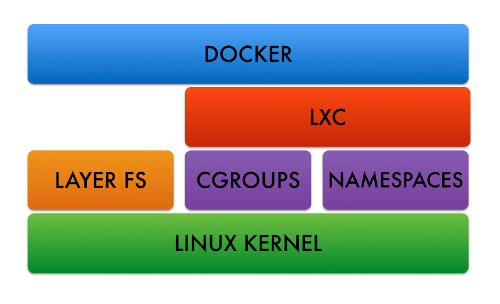
\includegraphics[scale=0.7]{pics/docker_arch.png}
	\caption{Wysokopoziomowe spojrzenie na architekturę systemu Docker.}
	\label{docker_arch}
\end{figure}

Na rysunku \ref{docker_arch} przedstawiono stos technologiczny rozwiązania Docker. Na samym dole stosu znajduje się serwer, czyli fizyczna maszyna na której uruchomiony jest system operacyjny. Ten uruchomiony system będzie służył do uruchamiania kontenerów i to jego zasoby będą wydzielane dla poszczególnych kontenerów. Na systemie hoście należy zainstalować pakiet docker-engine. Umożliwi to nam uruchamianie kontenerów z przygotowanych wcześniej obrazów, w których będą znajdowały się faktyczne aplikacje oraz wszystkie potrzebne tym aplikacjom biblioteki. Zaleca się aby uruchamiać tylko jedną aplikację w danym kontenerze. Ułatwia to chociażby wyciąganie logów z wnętrza kontenera, oraz odpowiedniemu wyizolowaniu aplikacji, gdyż zasoby możemy podać tyko dla konkretnego kontenera a nie dla każdego procesu. Tabela \ref{docker_cli} ukazuje listę komend rozwiązania docker wraz z krótkim opisem i przykładem użycia. Najważniejszymi z nich są \textit{run, stop, delete, ps, images, build oraz exec}. Pozwalają one przejść tzw. \textit{Container lifecycle}, czyli cykl życia kontenera – zbudowanie obrazu, uruchomienie go, wykonanie w nim jakiejś operacji oraz zatrzymanie a następnie usunięcie go.

\begin{table}[!htbp]
\caption{Ważniejsze polecenia w programie docker (dla wersji 1.13.1). \cite{ad27}}
\label{docker_cli}
\begin{tabular}{|p{3cm}|p{11cm}|}
  \hline
  \textbf{Polecenie} & \textbf{Opis oraz przykład}\\
  \hline
  docker attach & Podłączenie się do uruchomionego już kontenera, celem przechwycenia wyjścia z aplikacji uruchomionej w kontenerze. Kontener należy wskazać poprzez identyfikator lub nazwę (pole obowiązkowe). \newline docker attach world-community-grid \\
  \hline
  docker build & Zbudowanie kontenera w oparciu o podany plik Dockerfile. Narzędzie do budowania obrazów odszuka obraz który ma być podstawą dla naszego obrazu, a następnie wykona na nim wszystkie sekwencje wypisane w pliku Dockerfile. Ostatecznie na dysku zostanie zapisany gotowy do użycia obraz. O ile nie podamy parametru –tag jedynym sposobem na dostęp do obrazu będzie odwołanie się poprzez nadane ID.
  \newline docker build . -t  world-community-grid \newline Zakładając, że w bieżącym katalogu znajduje się poprawny plik Dockerfile, po uruchomieniu tej komendy zostanie on przetworzony. Zbudowany obraz otrzyma ID oraz zostanie otagowany jako  world-community-grid:latest \\
  \hline
  docker commit & Umożliwia stworzenie nowego obrazu w oparciu o już istniejący kontener lub obraz. \newline docker commit --change "ENV DEBUG true" c3f279d17e0a rsmitty/boinc \\
  \hline
  docker cp & Kopiuje pliki między kontenerem a systemem hostem i odwrotnie \newline docker cp /tmp/foo.txt world-community-grid:/tmp \\
  \hline
  docker create & Tworzy kontener na zasadzie identycznej jak docker run, z tą różnicą że kontener nie jest jeszcze uruchomiony i jego uruchomienie należy wykonać oddzielnie za pomocą docker start \newline docker create -t -i fedora bash \\
  \hline
  docker exec & Wykonuje podane polecenie we wskazanym kontenerze. Odpowiednie flagi decydują o lokalizacji wyjścia z podanego polecenia. \newline docker exec -it  world-community-grid bash \newline Uruchomi basha w kontenerze w sposób interaktywny. \\
  \hline
  docker images & Wyświetlanie listy obrazów pobranych i gotowych do użycia w systemie. \newline docker images –all \newline Wyświetlenie listy wszystkich obrazów znajdujących się na maszynie. \\
  \hline docker inspect & Wyświetlenie bardzo szczegółowych informacji na temat obrazu lub kontenera. \newline docker inspect  world-community-grid \\
  \hline docker ps & Wyświetlenie listy uruchomionych kontenerów. \newline docker ps -a \newline Wyświetli listę wszystkich kontenerów w systemie, nawet tych, które są zatrzymane bądź skończyły pracę. \\
  \hline docker pull & Pobieranie ze zdalnego repozytorium obrazów wskazanego obrazu \newline docker pull rsmitty/boinc \\
  \hline docker push & Opublikowanie na zewnętrznym repozytorium wskazanego obrazu obecnego w systemie \newline docker push rsmitty/boinc \\
  \hline docker rm & Usunięcie kontenera o wskazanej nazwie/ID \newline docker rm  world-community-grid \\
  \hline docker run & Stworzenie i uruchomienie kontera o określonych parametrach. \newline \newline docker run --restart=always -d --name wcg -e "boincurl=www.worldcommunitygrid.org" -e "boinckey=1033877\_ca3e3556f2fcafbb8edc82447e16b58c" rsmitty/boinc \newline Utworzy kontener z obrazu rsmitty/boinc (a jeśli taki nie jest obecny na dysku to docker podejmie próbę pobrania go). Do kontenera zostaną przekazane dwie zmienne środowiskowe i zostanie nadana mu nazwa world-community-grid.  \\
  \hline
\end{tabular}
\end{table}

 Nie trudno zauważyć, że w problemie konteneryzacji najważniejsze są dwa zagadnienia, tj. obsługa cyklu życia kontenera oraz zarządzanie obrazami. Obrazy dockerowe są trzymane w repozytoriach obrazów (ang. docker registry) a zarządzanie nimi odbywa się w sposób podobny do klasycznych repozytoriów kodu. W centrum danych można uruchomić takie repozytorium i przechowywać na nim obrazy. Dzięki temu zabiegowi wystarczy tylko raz zbudować obraz (co przy złożonych obrazach zajmuje wiele czasu) i po jego przesłaniu (polecenie docker push) można taki obraz pobrać (polecenie docker pull) na pozostałych serwerach w centrum danych.

 Obrazy w dokerze opierają się na plikach Dockerfile. Są to pliki tekstowe, w których musi zostać uwzględniona notacja Dockera oraz przygotowane dla użytkownika dyrektywy. Najważniejsze z nich to \textit{FROM, RUN}, oraz \textit{CMD}:

\begin{itemize}
\item Dyrektywa \textit{FROM} pozwala na wskazanie jaki obraz ma być podstawą dla opisywanego właśnie obrazu. Ta dyrektywa powinna pojawiać się na samym początku pliku Dockerfile.
\item \textit{RUN} pozwala na wykonywanie poleceń. Narzędzie do budowania obrazów uruchomi każdą komendę i jej wynik zapisze do „mini” obrazu (warstwy). Przy zakończeniu budowania wszystkie warstwy zostaną złączone w jeden obraz. To podejście ma ogromną zaletę: przebudowywanie komend raz już wykonanych jest szybkie, gdyż po prostu zostanie użyta zbudowana wcześniej warstwa. Przykładowy stos warstw obrazu pokazany jest na rysunku (Rys. \ref{docker_layers}).
\begin{figure}[ht!]
	\centering
	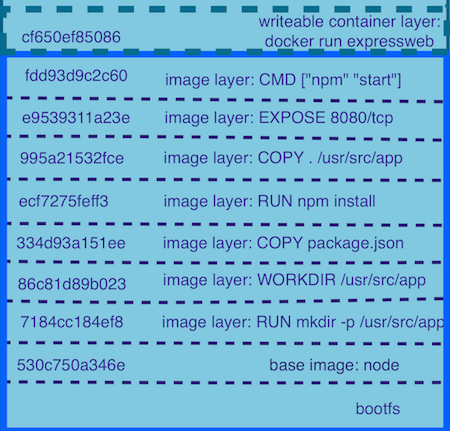
\includegraphics[scale=0.7]{pics/docker_layers.png}
	\caption{Lista warstw jakie składają się na obraz ‘expressweb’.}
	\label{docker_layers}
\end{figure}
\item \textit{CMD} określa komendę jaka zostanie uruchomiona przy starcie kontenera. Poprawne ustawienie tego polecenia jest kluczowe dla właściwego działania aplikacji. To właśnie logi tego polecenia będą znajdowały się na wyjściu polecenia docker logs.
\end{itemize}

W związku z tym, że nie każdy użytkownik ma zestawione swoje repozytorium firma docker uruchomiła swoje własne \cite{ad28}, które jest dostępne w Internecie. Prócz repozytorium obrazów jest dostępny też web serwis, który w przyjaznej formie prezentuje wszystkie informacje. Produkt jest dostępny pod adresem https://hub.docker.com

\begin{figure}[!h]
	\centering
	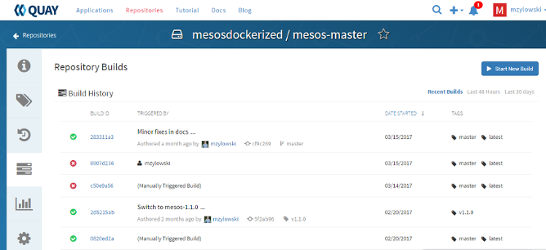
\includegraphics[scale=1]{pics/quay.png}
	\caption{Historia przebudowywania obrazu mesos-master napisanego na potrzeby tej pracy.}
	\label{quay_io}
\end{figure}

Ze względu na monopol dockera pojawił się projekt wspierający inne formaty obrazów. Mowa tutaj o repozytorium i web serwisie dostępnym pod adresem https://quay.io \cite{ad28}. Na rysunku \ref{quay_io} widoczny jest zrzut ekranu z serwisu quay.io.

\subsection{Rozwiązanie konteneryzacyjne \textit{rkt}}

\begin{figure}[!h]
	\centering
	
\includegraphics[scale=1]{pics/rkt-horizontal-color.png}
	\caption{Logo projektu rkt.}
	\label{rkt_logo}
\end{figure}

Rkt \cite{ad29}(Rys. \ref{rkt_logo}) jest produktem sponsorowanym przez firmę CoreOS i jest próbą wydarcia części rynku Dockerowi. Rkt jest aplikacją pozwalającą uruchamiać kontenery na systemach z rodziny Linux, a celem przyświecającym twórcom aplikacji było zaprojektowanie jej tak by \cite{ad29}:

\begin{itemize}
\item Bazowała na \textit{podach} - \textit{pod} to byt tworzacy przestrzeń do uruchamiania w sobie wielu kontenerów. Ułatwia to łączenie aplikacji między sobą i ich organizowanie. Kontenery realizujące zadania ze sobą powiązane mogą być trzymane w jednym podzie, co dodatkowo oddziela je od innych zadań w systemie. Zadania w jednym podzie mogą interferować między sobą. \textit{Pod} można rozumieć jako kolejną wartstę abstrakcji oddzielająca procesy uruchomione przez system operacyjny.
\item Zapewniała bezpieczeństwo bez żadnych dodatkowych konfiguracji - natywne wsparcie dla mechanizmu \textit{SELinux} oraz uruchamianie aplikacji w maszynach wirtualnych.
\item Integrowała się z innymi systemami związanymi z uruchamianiem zadań (\textit{systemd}, \textit{upstart}) oraz z orkiestratorami zadań na klastrach (\textit{Kubernetes}, \textit{Nomad}).
\item Wspierała i zachowywała standardy dotyczące konteneryzacji oraz współpracowała z istniejącymi formatami obrazów. Rkt potrafi uruchomić obraz w specyfikacji \textit{OCI} lub obraz zbudowany oprogramowaniem docker. Produkt wykorzystuje rozwiązania projektu \textit{Container Networking Interface}, który rozwiązuje problem sieci między uruchomionymi kontenerami.
\end{itemize}

\begin{figure}[!h]
	\centering
	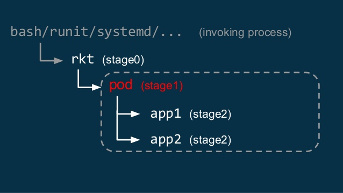
\includegraphics[scale=1]{pics/rkt-architecure.jpg}
	\caption{Architektura rozwiązania rkt.}
	\label{rkt_arch}
\end{figure}

Rozwiązanie rkt bazuje na tak zwanych ang. \textit{stage} \cite{ad30}. Pozwalają one na wyraźne rozgraniczanie poszczególnych modułów systemów co umożliwia wprowadzenie warstwowej podmienialnej architektury całego rozwiązania. Na rysunku \ref{rkt_arch} przedstawiono architekturę tego rozwiązania (przy uruchomionym jednym podzie i dwóch kontenerach). I tak \cite{ad30}:

\begin{itemize}
\item stage0 - jest to poziom systemu operacyjnego i procesu samej aplikacji rkt.
\item stage1 - jest to poziom poda, swego rodzaju baza dla dalszego uruchamiania kontenerów. Stage1 to bardzo mocno okrojony system plików, który umożliwia uruchamianie prostych aplikacji i ploleceń systemu operacyjnego. W tym miejscu uwidacznia się jedna z największych sił rozwiązania rkt. Stage pierwszy może być podmieniany (jest tak naprawdę obrazem systemu plików). W zależności od wskazanego obrazu określimy sposób w jaki rkt będzie dokonywał izolowania uruchomionych później kontenerów. Aktualnie wraz z rozwiązaniem dostarczanych jest pięć obrazów, które mogą być tutaj wykorzystane (tabela \ref{rkt_flavors}).
\item stage2 - jest to poziom aplikacji uruchomionej w kontenerze. Wskazany obraz zostaje uruchomiony za pomocą odpowiedniego \textit{hypervizora}.
\end{itemize}

\begin{table}[!htbp]
\caption{Lista obrazów, które mogą być użyte jako stage1 w systemie konteneryzacji rkt. \cite{ad30}}
\label{rkt_flavors}
\centering
\begin{tabular}{|p{3cm}|p{3cm}|p{8cm}|}
  \hline
  \textbf{Nazwa rozwiązania} & \textbf{Wykorzystywany mechanizm izolacji} & \textbf{Opis mechanizmu izolacji}\\
  \hline
  Fly & System plików i polecenie chroot & Ten mechanizm izolacji polega na skopiowaniu zawartości obrazu do innej lokalizacji a następnie wykonaniu tam polecenia chroot. W tym podejściu nie istnieje w zasadzie izolacja procesów uruchomionych w kontenerze. Będą one interferowały inne aplikacje uruchomione w systemie operacyjnym. Jedynym zystkiem z tej izolacji uniemożliwieniu użytkownikowi wyjście poza kontener (ucieczka do systemu gospodarza). \\
  \hline
  Rkt stage1 & systemd-nspawn, cgroups & Domyślny mechanizm izolacji stosowany w rkt. Zostanie wykorzystany jeśli parametr --stage1-name nie zostanie podany do polecenia uruchamiającego kontener. Jest to mechanizm analogiczny do już wcześniej opisanego sposobu izolacji wykorzystywanego w Dokerze. Podobnie jak w mechaniźmie \textit{Fly} zawartość obrazu jest rozpakowywana do lokalizacji w systemie operacyjnym a następnie polecenie chroot więzi użytkownika w odpowiednim katalogu. W tym rozwiązaniu jednak procesy kontenera są izolowane za pomocą mechanizm \textit{cgroup} (analogicznie jak w dokerze). \\
  \hline
  LKVM & Wirtualizacja KVM & To podejście jest kolejnym wyróżnikiem rkt. LKVM (\textit{lightweight} KVM) to niewielka aplikacja, która umożliwa uruchamianie maszyn wirtualnych wykorzystując sprzętowe technologie wirtualizacyjne. Dla procesorów AMD jest to technologia AMD-V, zaś dla procesorów rodziny intel Intel VT-x. Uruchomienie kontenera za pomocą programu LKVM to w zasadzie uruchomienie prostej maszyni wirtualnej. To podejście zapewnia wysoki poziom izolacji. \\
  \hline
  QEMU & Wirtualizacja KVM & Projekt LKVM w swoich założeniach miał być projektem lekkim, co wraz z rozwojem projektu rkt rodziło wiele problemów. Latem 2016 roku podjęto decyzje by zaimplementować konteneryzację wykorzystując technologię QEMU \cite{ad31}. QEMU jest rozwiązaniem bardzo rozbudowanym - umożliwia zarówno wykorzystanie emulacji sprzętowej jak i technologi KVM. Przez złożoność rozwiązania doszło do znaczącego spadku wydajności i wkrótce quemu zostało zastąpione pakietem quemu-lite \cite{ad32}. \\
  \hline
  XEN & Wirtualizacja XEN & Zewnętrzni klienci produktu rkt aby wypromować swoje rozwiązanie przygotowali stage1 oparty na wirtualizacji XEN. Na dzień pisania tej pracy projekt jest w fazie rozwojowej i nie jest używalny produkcyjnie. \\
  \hline
\end{tabular}
\end{table}

\newpage

\section{Orkiestratory zadań}

\subsection{Apach Mesos}

Produkt \cite{ad34} \ref{mesos_logo} \textit{open source} przeznaczony do instalacji w centrum danych oferujący możliwość uruchamiania zadań na zadanych zasobach. Rozwijany początkowo na Uniwerystecie w Berkeley. Pierwsza prezentacja Mesosa miała miejsce w 2009 roku podczas konferencji \textit{HotCloud}. Projektem zainteresowała się fundacja Apache, która do dnia dzisiejszego zajmuje się rozwojem produktu. W Lipcu 2016 została wydana wersja 1.0 Mesosa (przeskok z wersji 0.26). Na ten krok zdecydowano się po zaimplementowaniu wielu dodatkowych funkcji, po dołączeniu do projektu firmy Mesosphera. Tak przygotowany produkt firma Mesosphera zaczęła rozprowadzać pod swoim logo jako kompleny produkt pozwalający osiągnąć wysoką utylizację centrum danych. Mowa tutaj o produkcie DC/OS \textit{Data Center Operating System}. 

\begin{figure}[!h]
	\centering
	
\includegraphics[scale=1]{pics/apache_mesos_logo.png}
	\caption{Logo projektu Apache Mesos.}
	\label{mesos_logo}
\end{figure}

Mesos architektonicznie \cite{ad33} jest projektem, który zbiera zasoby ze wszystkich komputerów na których jest uruchomiony i przedstawia ją jako zunifikowaną pulę. Następnie pula ta może być użyta do uruchomienia zadań. Do zebranych zasobów należy się odwołać używając bądź implementując własny \textit{framework}. W tym miejscu uwidacznia się siła rozwiązania, ponieważ niewielkim wysiłkiem można zaprojektować swoje własne rozwiązanie, które będzie efektywnie rozdzielało zadania do wykonania. Umożliwia to specjalne programowe API, które wystawia Mesos.

Mesos początkowo wszystkie zadania uruchamiał jako kolejne procesy na wybranej do egzekucji maszynie. To podejście było bardzo prostą izolacją, która dopiero później była dalej rozwijana. Również procesy odpowiedzialne za działanie Mesosa były uruchamiane jako zwykłe procesy, tak więc zadanie uruchomione w Mesosie mogło w skrajnej sytuacji interferować nawet proces samego kontrolera klastra. Popoularność rozwiązania Docker sprawiła, że do Mesosa dodano możliwość uruchomienia skonteneryzowanych aplikacji. Dodatkowo zaleca się uruchomienie poszczególnych procesów dockera w osobnych kontenerach, w ten sposób wszystkie uruchomione zadania są od siebie izolowane i nie interferują procesów samego Mesosa.

Na dzień pisania tej pracy Mesos posiada tylko eksperymentalne wsparcie dla kontenerów \textit{appc}. Nie jest możliwe uruchamianie wielu kontenerów w jednym podzie, a samo wspracie dla rkt nie jest stabilne. Przyczyną tego stanu rzeczy jest niechęć firmy Mesosphera do wspierania produktu konkurencyjnego dla Dokera i prawdopodobnie tak długo jak rkt nie zdobędzie większej popularności, tak długo Mesos nie będzie posiadał produkcyjnego wsparcia dla wszystkich mechanizmów, które oferuje rkt.

Architektura Mesosa oraz istniejące na rynku \textit{frameworki} zostały opisane w kolejnym rozdziale tej pracy. 

\subsection{Kubernetes}

Kubernetes \cite{ad35}(rys. \ref{kube_logo}) - znacznie młodsza konkurencja rozwiązania Mesos (po raz pierwszy ogłoszony publicznie w połowie roku 2014). Sponsorowany i rozwijany jako wolne oprogramowanie przez korporację Google. Rozwiązanie od samego początku oparte było o kontenery Dockera. Nigdy nie powstała możliwość uruchamiania pojedyńczych procesów w systemie operacyjnym (tak jak w Mesosie). Kubernetes jako rozwiązanie młode często wprowadza zmiany architektoniczne i nowe możliwości. Jego niedojrzałość powoduje, że trzeba włożyć więcej pracy w aktualizacje klastra i zapewnienie stabilności. Przykładem zmiany, która doprowadziła do takich problemów może być mechanizm CRI \textit{Container Runtime Interface}. Ze względu na pojawiające się konkurencyjne do Dokera rozwiązania kontenerowe (rkt, OCI) w kubernetesie zaprojektowano mechanizm CRI. Jest to programowe API działające po specjalnie przygotowanej przez Google implementacji protokołu RPC - GRPC. Dany \textit{runtime} kontenerowy musi implementować to API by porozumiewać się z kubernetesem. Rozwiązania kontenerowe zaprojektowały swoje odzielne procesy, których celem była komunikacja po interfejsie CRI. Dla rkt jest to proces \textit{rktlet} a dla Dockera \textit{docker-shim}. Zainstalowanie wersji 1.6 wymagało również aktualizację konteneryzatora, a to wymagało wyłączenia bądź przemigrowania usług działających na danym komputerze w klastrze. Porównanie architektury kubernetesa 1.5 z 1.6 przedstawiono odpowiednie na rysunkach \ref{k8s_1_5} i \ref{k8s_1_6}. Dodatkowo na rysunku \ref{k8s_1_6} widoczne są zmiany związne z dodaniem interfejsu CRI.

\begin{figure}[!h]
	\centering
	
\includegraphics[scale=1]{pics/Kubernetes-logo.png}
	\caption{Logo projektu Kubernetes.}
	\label{kube_logo}
\end{figure}

Architektonicznie \cite{ad36}(Rys. \ref{k8s_1_6}) kubernetes jest mocno złożoną aplikacją. Poszczególne elementy aplikacji zostały porozdzielane na osobne usługi a nie jak w przypadku Mesosa zamknięte niemal w dwóch usługach. Wyróżnić należy szczególnie proces \textit{kubelet}, który jest sercem całego rozwiązania. Każdy komputer na którym uruchomiony jest proces kubeleta należy do klastra kubernetesa. Jest to jedny proces, który należy uruchomić z poziomu systemd. Wszystkie inne potrzebne procesy zostaną uruchomione jako byty kubernetesa (jako kontenery). Sam kubelet również może być uruchomiony w kontenerze, co jest domyślnym ustawieniem gdy klaster jest instalowany z narzędzia \textit{kubespray}. 

\begin{figure}[!h]
	\centering
	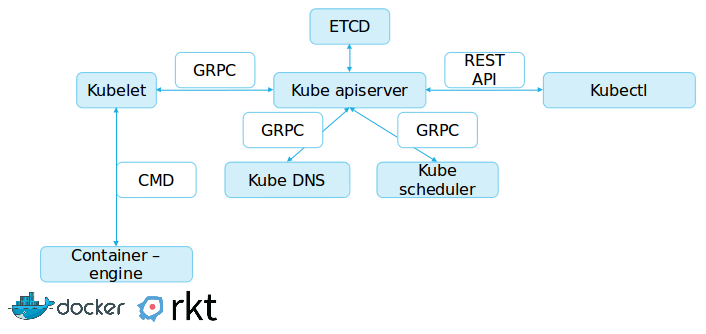
\includegraphics[scale=0.7]{pics/k8s_1_5.png}
	\caption{Architektura projektu Kubernetes w wersji 1.5.}
	\label{k8s_1_5}
\end{figure}

\begin{figure}[!h]
	\centering
	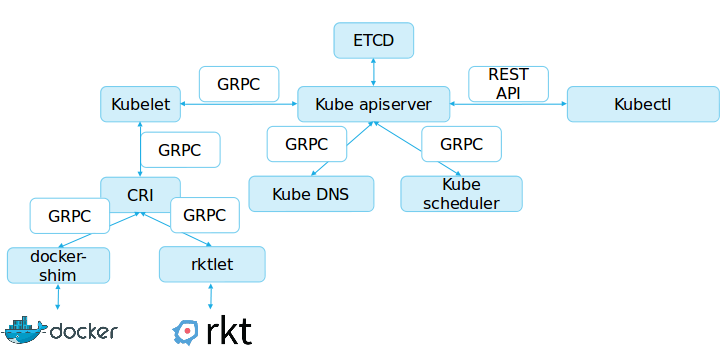
\includegraphics[scale=0.7]{pics/k8s_1_6.png}
	\caption{Architektura projektu Kubernetes w wersji 1.6.}
	\label{k8s_1_6}
\end{figure}

Usługi w stosie architektonicznym kubernetesa komunikują się za pomocą protokołu GRPC. Wyjątkiem jest jedynie aplikacja \textit{kubectl}, która to komunikuje się z klastem za pomocą technologi REST API. \textit{Kubectl} jest programem pozwalającym komunikować się i zarządzać klastrem z poziomu konsoli \textit{bash}.

Prócz \textit{kubelet'a} i \textit{kubectl'a} do poprawnego działania klastra potrzebne są inne procesy (Rys. \ref{k8s_1_6}, \ref{k8s_1_5}):
\begin{itemize}
\item Kube-apiserver - Aplikacja, która pośredniczy między klastrem a użytkownikiem. Potrafi komunikować się z innymi procesami w klastrze za pomocą protokołu GRPC jednocześnie wystawiając HTTP REST API, dzięki któremu aplikacje takie jak kubectl są w stanie łączyć się z klastrem i wykonywać na nim polecenia. Korzystając w tym miejscu z protkołu HTTPS skorzystano ze wszystkich dobrodziejstw tego protokołu - szyfrowanie, połączenia w oparciu o certyfikaty czy klucze. Umożliwia to łatwe zarządzanie uprawnieniami - użytkownikowi, który powinien posiadać możliwość zarządzania klastrem, należy dostarczyć odpowiedni certyfikat.
\item Kube-dashboard (Rys. \ref{k8s_dash}) - jest to opcjonalna aplikacja, która może zostać zainstalowana wraz z klastrem. Umożliwia ona zarządzanie klastrem z wykorzystaniem przeglądarki internetowej. Oferuje znacznie mniej możliwości niż kubectl, natomiast dobrze nadaje się do zastosowań monitoringu czy też uruchamiania zadań przez niedoświadczonych użytkowników. Kube-dashboard również komunikuje się z klastrem wykorzystując API uruchomione przez kube-apiserver.
\begin{figure}[!h]
	\centering
	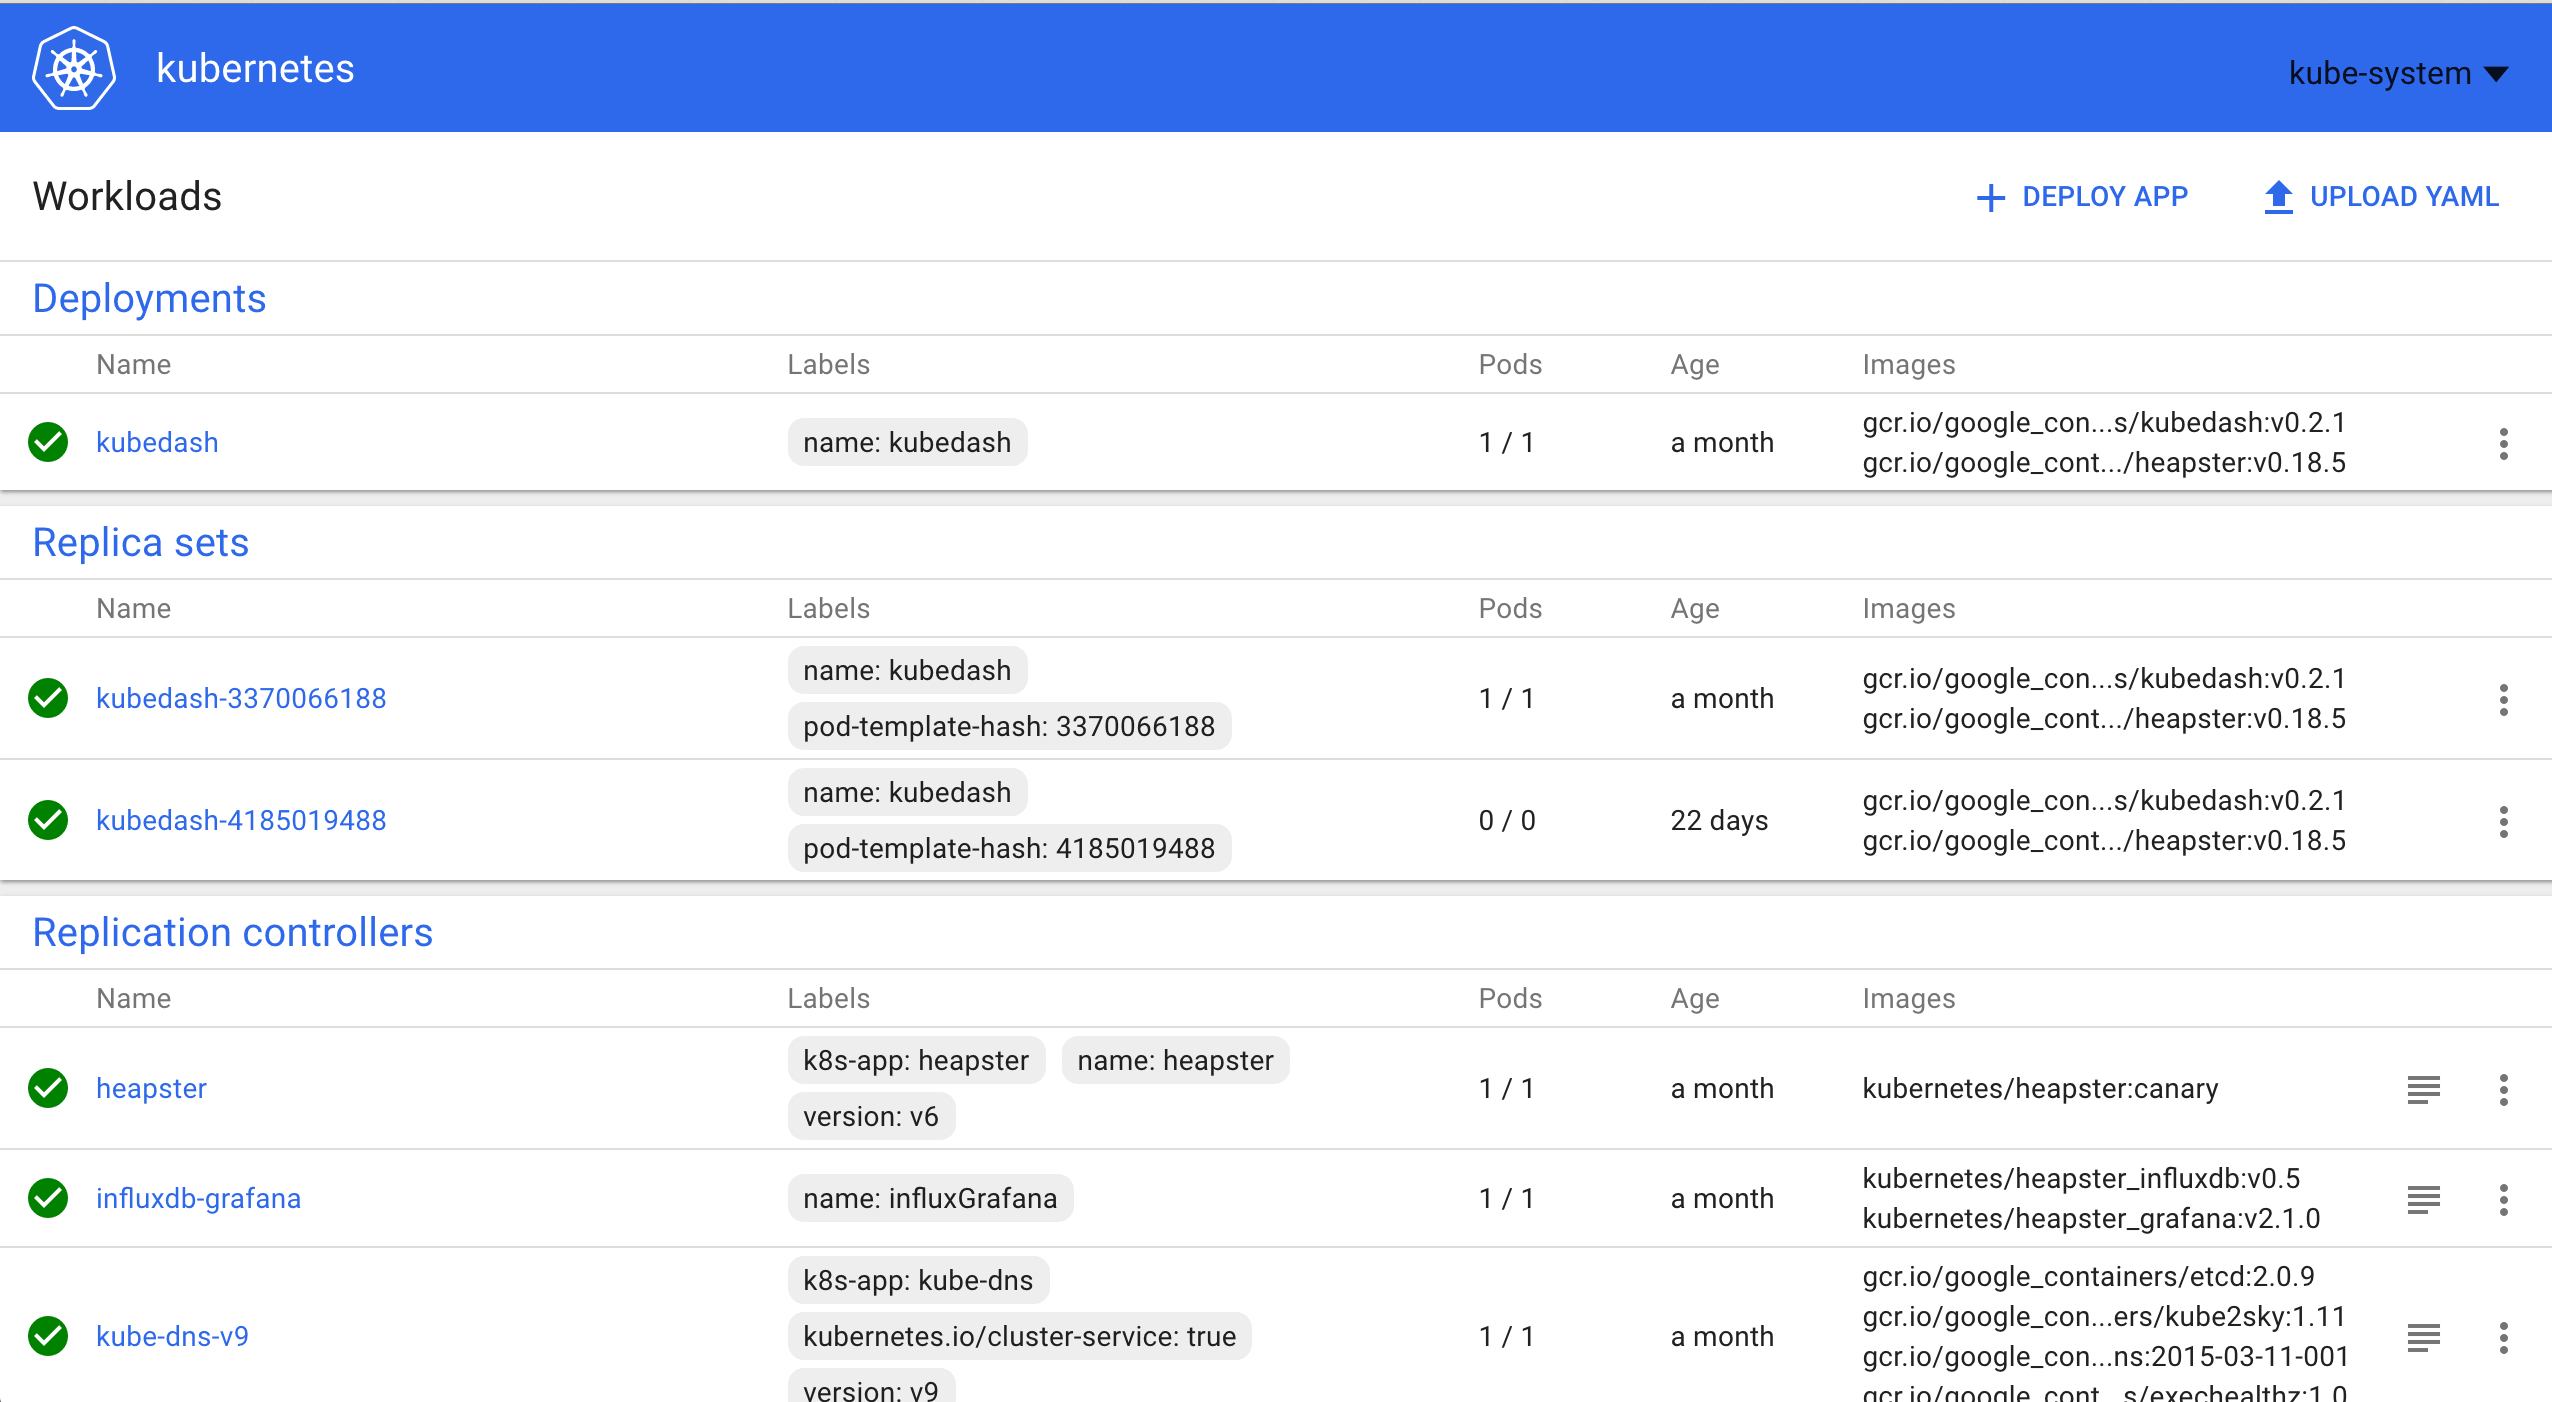
\includegraphics[scale=0.17]{pics/kubedash.png}
	\caption{Zrzut ekranu z aplikacji kube-dashboard.}
	\label{k8s_dash}
\end{figure}
\item Etcd \cite{ad37} - jest to baza danych, która jest wykorzystywana przez klaster kubernetesa do przechowywania informacji na temat stanu klastra. Etcd jest projektem rozwijanym niezależnie od kubernetesa przez firmę CoreOS. Jest to nie relacyjna baza danych, która dane przechowuje w postaci: klucz - wartość. Etcd posiada możliwość sklastrowania swoich uruchomionych instancji, co zapewnia bezpieczeńtwo i niezawodność w przypadku awarii jednego z komputerów w klastrze.
\item Kube-scheduler - proces, który odpowiedzialny jest za rozkładanie zadań pomiędzy poszczególne komputery klastra. Aplikacja tylko w niewielkim stopniu jest konfigurowalna, zaś sam algorytm rozdzielania zadań jest zamknięty wewnątrz aplikacji i nie ma możliwości dostosowania go do własnych potrzeb. Kube-scheduler decyzję o kolejkowaniu zadań na poszczególne komputery w klastrze oprze o tak zwane etykiety ang. \textit{labels}. Etykiety są opcjonalnym mechanizmem. Pozwalają one grupować poszczególe komputery klastra. Przykładowo komputery z dużą ilością dysków twardych mogą być oznaczone odpowiednią etykietą. Następnie uruchamiając zadanie, które wymaga wygenerowania dużej ilości danych, poprzez odpowiednią etykietę, może być skierowane właśnie na taki komputer. Do problemu rozdzielania zadań, wrócę jeszcze w kolejnym rozdziale, gdzie zostaną porównane możliwości Kubernetesa i Mesosa \ref{k8s_mesos_comparision}.
\item Kube-dns - odpowiedzialny jest za komunikację sieciową z zewnątrz klastra do aplikacji uruchomionych wewnątrz. Mechanizm ten umożliwia uruchamianie na klastrze serwisów, które mają być dostępne z zewnątrz (np. strony internetowe, bazy danych). Do komunikacji wewnętrznej w klastrze wykorzystywane są plug-in'y sieciowe, które nie będą szczegółowo opisywane w tej pracy.
\end{itemize}

\newgeometry{top=2.5cm, bottom=2.5cm, left=2.5cm, right=3.5cm}
\onehalfspacing
\chapter{Analiza rozwiązania Mesos oraz przegląd systemów szeregowania zadań}

\section{Architektura rozwiązania Mesos}

Mesos (Rys. \ref{mesos_logo}) zaprojektowany jest w oparciu o dwie aplikacje napisane w języku C++. Są to \textit{mesos-master} i \textit{mesos-agent}. Zasoby każdego komputera, na którym zostanie uruchomiona aplikacja \textit{mesos-agent} zostaną zaraportowane do uruchomionej na innym komputerze aplikacji \textit{mesos-master}. Master pozwala uruchamiać zadania na zadanej puli poprzez wystawienie programowego API. API to musi zostać zaimplementowane przez aplikację \textit{framework}, która uzyska możliwość uruchamiania zadań na puli zasobów mastera. Jednocześnie implementując \textit{framework} implementuje się sposób rozdzielania zadań na klastrze, dlatego właśnie w kontekście Mesos'a określenie \textit{framework} stosuje się wymienie ze słowem \textit{scheduler}. Warto tutaj zaznaczyć, że do uruchomienia Mesosa wystarczy nawet jeden komputer. Master i Agent mogą koegzystować na jednym komputerze. Uruchomienie jednego frameworka jest wystarczające do uruchamiania zadań. 

\textit{Schedulerów} do Mesos'a dostępnych jest sporo, więc często nie ma konieczności implementowania własnego rozwiązania. Wiele projektów związanych z chmurami obliczeniowymi przygotowywało własne \textit{frameworki}, tak aby zachęcić właścicieli infrastrutury do łatwej integracji obecnych rozwiązań z Mesosem.

\subsection{Cykl życia zadania}

Przebieg zadania w klastrze Mesos'a prezentuje się następująco:
\begin{enumerate}
\item Użytkownik klastra zleca zadanie do wykonania. Zlecenie następuje poprzez \textit{frameworki} zarejestrowany w Mesosie. 
\item Zadanie zostaje przekazane do procesu \textit{mesos-master} wraz z informacją na którym komputerze klastra zadanie ma zostać uruchomione.
\item Master przekazuje wszystkie informacje do procesu \textit{mesos-agent} na odpowiednim komputerze.
\item Aplikacja \textit{mesos-agent} uruchamia komponent \textit{mesos-egzecutor}, który odpowiedzialny jest za uruchomienie zadania. 
\item \textit{Mesos-egzecutor} przed uruchomieniem zadania wykonuje szereg czynności, takich jak rezerwacja zasobów, pobranie wskazanych w zadaniu elementów itd.
\item Gdy cała przestrzeń do wykonania zadania jest przygotowana, zostaje uruchomiony właściwy proces. 
\item Przez cały czas trwania zadania występuje wymiana informacji między aplikacjimi \textit{mesos-agent}, \textit{mesos-master} i \textit{schedulerem}. Zostaje również zaktualizowana informacja na temat dostępnych zasobów.
\item Zadanie kończy się, a zasoby po zadaniu zostają zwolnione.
\end{enumerate}

\subsection{Tryb wysokiej dostępności}
Mesos przygotowany jest działania w trybie HA (ang. \textit{High Availability}). Pojawia się tutaj kolejna aplikacja która musi zostać zainstalowana na klastrze. Jest nią \textit{Zookeeper}. \textit{Zookeeper} jest odpowiedzialny, za przechowywanie informacji o położeniu wszystkich \textit{masterów} w klastrze. Dodatkowo sam \textit{Zookeeper} jest uruchomiony na wielu komputerach klastra, tak aby informacje o masterach były powielane na wielu komputerach. Niektóre frameworki dostępne na rynku uruchamiają się również w trybie HA, podobnie jak master wykorzystując mechanizm \textit{Zookeepera}. W przypadku konfiguracji wielu masterów zawsze tylko jeden jest liderem, zaś pozostałe są instancjami "awaryjnymi". 

W przypadku braku komunikacji z aktualnym liderem klastra:
\begin{enumerate}
\item Zookeeper tworzy listę wszystkich masterów podłączonych w klastrze.
\item Następuje wybór nowego lidra klastra.
\item Informacja o nowym liderze przesyłana jest do wszystkich masterów.
\item Wszystkie instancje frameworków i agentów na klastrze raportują swój stan, tak aby wszystkie zdarzenia przez nieobecność mastera, zostały odpowiednio przetworzone i zalogowane.
\item Nowy lider przejmuje kontrolę nad klastrem.
\end{enumerate}

Architekturę trybu HA przedstawiono na rys. (\ref{mesos-ha-arch}). Jest to przykładowy klaster, na którym działają 3 agenty (\textit{slaves}) oraz trzy komputery pełniące rolę mastera, wraz z zainstalowanym na nim \textit{zookeeperem}. 
\begin{figure}[!h]
	\centering
	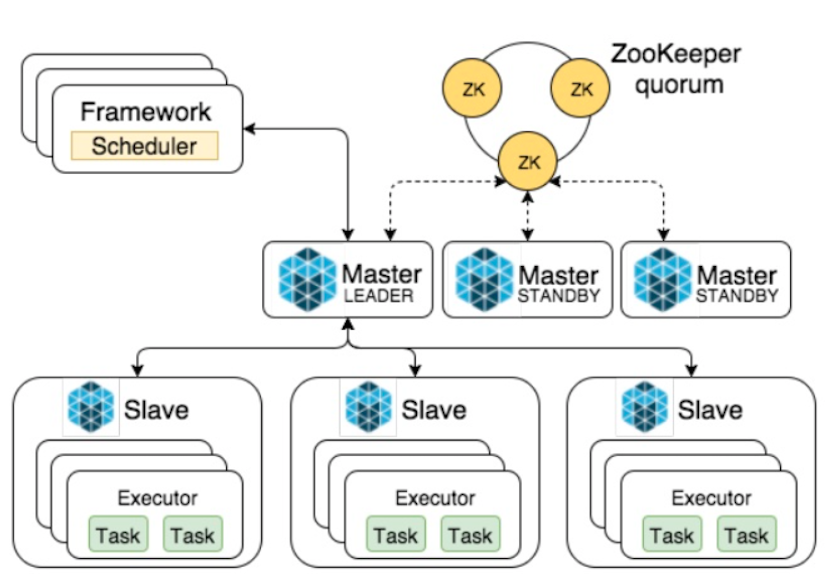
\includegraphics[scale=0.5]{pics/mesos-ha-arch.png}
	\caption{Klaster Mesos'a w trybie wysokiej dostępności.}
	\label{mesos-ha-arch}
\end{figure}

\subsection{Rozszerzalność Mesosa poprzez moduły}

Podobnie jak w przypadku \textit{frameworków}, Mesos wystawia programowe API, które umożliwia napisanie własnych modułów i podłączenie ich do klastra \cite{ad40}. Moduły mogą być używane zarówno z masterami jak i agentami. Rodzaje wspieranych w Mesosie modułów:

\begin{itemize}
\item Alokatory - pozwalają na zaimplementowanie zaawansowanych algorytmów przydzielania zasobów poszczególnym zadaniom. Przykładowo, można zaimplementować tutaj alokowanie pamięci z rożnych kości RAM, czy też używania dla poszczególnych zadań innych rodzajów dysków. Np. zadania wymagające przechowywania danych można uruchamiać na dyskach NVMe, zaś zadania obliczeniowe, które w niewielkim stopniu korzystają z dysku twardego, można uruchomić na przestrzeni dysku SATA.
\item Moduły anonimowe - nie są związane, z żadną dodatkową funkcjonalnością. Służą do uruchamiania własnego kodu przez procesy Mesos'a. Przykładowym modułem może tutaj być moduł do logowania lub monitorowania klastra.
\item Autentykatory - pozwalają na zaimplementowania systemu autentykacji na klastrze. System taki może wykorzystać mechanizmy takie jak LDAP czy NIS, bądź też oprzeć się całkowicie na własnym rozwiązaniu i trzymać dane użytkowników w bazie danych MySQL lub w szyfrowanych plikach.
\item Wyzwalacze (ang. \textit{Hooks}) - umożliwiają wykonywanie własnych dodatkowych akcji, po wykryciu danego zdarzenia. Przykładowo można tutaj zaprogramować mechanizm wysyłający wiadomości \textit{e-mail} po każdym uruchomionym zadaniu.
\item Izolatory - pozwalają na zaimplementowanie systemów związanych z izolowaniem zadań od siebie, czy też reagowania na sytuacje w których jedno zadanie jest interferowane przez drugie. Przykładem może być implementacja mechanizmu pozwalającego na migrowanie zadań z maszyn, na których zaczyna brakować zasobów z powodu innego trudnego obliczeniowo problemu.
\item Moduły elekcyjne - pozwalają zaimplementować własny mechanizm wybierania lidera po rozłączeniu poprzedniego. Można tutaj wykorzystać inną bazę danych niż tą oferowaną przez \textit{Zookeeper'a}, np. \text{ETCD}.
\end{itemize}

\subsection{Instalacja klastra}
Mesos \cite{ad33} \cite{ad34} w przeciwieństwie do kubernetesa nie posiada instalatora wskazywanego przez twórców rozwiązania. (Wyjątkiem jest tutaj komercyjna wersja - DC/OS). Kubernetes zaleca aby produkcyjne instalacje uruchamiane były w oparciu o kontenery. Jedyną aplikacją, która nie jest skonteneryzowana powinien być kubectl. Co więcej kubelet jest jedyną aplikacją, która uruchomiona jest w kotenerze bezpośrednio z poziomu systemd. Wszystkie pozostałe komponenty uruchamiane są już jako byty kubernetesa. W przypadku Mesos'a można zaobserwować znacznie bardziej tradycyjne podejście. Zalecaną metodą instalacji jest instalacja z paczek udostępnionych w repozytorium firmy \textit{mesosphere}. Skonfigurują się wtedy wszystkie \textit{unity systemd}, a na użytkowniku pozostanie jedynie kwestia umieszczenia adresów IP pozostałych elementów klastra. Niewątpliwie jednak, warto skorzystać z dobrodziejstw oferowanych przez izolację jaką dają kontenery i uruchomić klaster Mesosa z wykorzystaniem np technologii Docker. Jednym z podejść jest próba aplikowania obrazów przygotowywanych na potrzeby rozwiązania DC/OS. Innym skorzystanie z obrazów przygotowywanych przez innych użytkowników w ramach rozwoju wolnego oprogramowania. Ze względu na brak rozwiązania, które zadowalałoby mnie całkowicie postanowiłem w ramach tej pracy przygotować własne obrazy aplikacji \textit{mesos-master} oraz \textit{mesos-agent}. Więcej o tym produkcie napiszę w rozdziale 4.1.2.

\section{Interfejs i konfiguracja}
\subsection{Mesos HTTP API}
Prócz programowego API, które może zostać wykorzystane do tworzenia modułów i systemów szeregowania, Mesos udostępnia również HTTP REST API \cite{ad38}, które służy jednak głównie celom monitoringu klastra. Lista wybranych \textit{endpointów} znajduje się w tabli \ref{mesos_endpoints}.  Kilka endpointów zostało wykorzystanych do badań opisaych w rozdziale czwartym. 

\begin{table}[!htbp]
\caption{Lista \textit{endpointów} dostępnych w rozwiązaniu Mesos \cite{ad38}.}
\label{mesos_endpoints}
\centering
\begin{tabular}{|p{4cm}|p{10cm}|}
  \hline
  \textbf{\textit{Endpoint}} & \textbf{Realizowana funkcja} \\
  \hline
  /logging/toggle & Pozwala na zmianę poziomu logowania aplikacji przez określony zadany czas. Może być wykorzystany do dokładnego analizowania sytuacji na klastrze.\\
  \hline
  /master/create-volumes & Tworzy wolumen, który może być później wykorzystany na potrzeby zadania. Do utworzenia wolumenu konieczne jest wskazanie agenta na którym wolumen powinien zostać stworzony. \\
  \hline
  /master/destroy-volumes & Niszczy wcześniej stworzony wolumen. \\
  \hline
  /master/frameworks & Wyświetla listę i informacje o zarejestrowanych \textit{frameworkach}. \\
  \hline
  /master/health & Zwraca informacje o zdrowiu wskazanego master'a. Jeśli reakcje master'a będą wolne lub będą inne problemy na podanym serwerze, to odpowiednia informacja zostanie tutaj zwrócona. \\
  \hline
  /maintenance/schedule & Pozwala ustawić klaster w tryb konserwacji. Umożliwia to wyłączanie wskazanych maszyn z klastra, celem wykonania fizycznych manipulacji przy sprzęcie, bądź innych prac administracyjnych w systemie. \\
  \hline
  /redirect & Zwraca informacje, który master jest aktualnym liderem. \\
  \hline
  /master/slaves & Pozwala na uzyskanie informacji oraz adresów IP podłączonych do klastra agentów. \\
  \hline
  /master/state & Zwraca stan wskazanego mastera. Odpowiedź zostanie zwrócona w formacie JSON. Będzie to wiele danych, począwszy od czasu elekcji, poprzez flagi z jakimi uruchomiony był master, na zarejestrowanych agentach skończywszy. Listę ważniejszych flag konfiguracyjnych umieszczono w tabeli \ref{mesos_flags}. \\
  \hline
  /tasks & Wyświetla informacje o wszystkich zadaniach na klastrze, ze wszystkich zarejestrowanych frameworków. \\
  \hline
  /teardown & Wyłącza wskazany framework, po wcześniejszym przymusowym zakończeniu wszystkich zadań na nim uruchomionym. \\
  \hline
  /metrics/snapshot & Zrzuca wszystkie mierzalne w Mesosie metryki w chwili wywołania do pliku, celem późniejszej analizy. Lista ważniejszych metryk została przedstawiona w tabeli \ref{mesos_metrics}.\\
  \hline
  /profiler/start & Uruchamia wbudowany w Mesosa system do profilowania pamięci. \\
  \hline
  /profiler/stop & Wyłącza tryb profilowania i zapisuje wynik do pliku. \\
  \hline
\end{tabular}
\end{table}

\subsection{Monitoring klastra za pomocą oferowanych przez Mesos'a metryk}
Problem monitoringu klastra jest jedynm z ważniejszych, z jakich muszą sobie poradzić administratorzy DC. Wiele dostępnych narzędzi umożliwia przygotowanie zaawansowanych widoków i wykresów, które wykorzystują odpowiednie skrypty i odpytują system operacyjny o metryki. W przypadku Mesos'a część metryk udostępniona jest poprzez API \ref{mesos_metrics}.

\begin{table}[!htbp]
\caption{Lista metryk związanych z zasobami, dostępnych w rozwiązaniu Mesos \cite{ad39}.}
\label{mesos_metrics}
\centering
\begin{tabular}{|p{4cm}|p{10cm}|}
  \hline
  \textbf{Metryka} & \textbf{Opis} \\
  \hline
  master/cpus\_percent & Procent zaalokowanych procesorów.\\
  \hline
  master/cpus\_used & Ilość zaalokowanych procesorów. \\
  \hline
  master/cpus\_total & Całkowita liczba procesorów. \\
  \hline
  master/disk\_percent & Procent zaalokowanej przestrzeni dyskowej. \\
  \hline
  master/disk\_used & Zaalokowana przestrzeń dyskowa. Zwracana w mega bajtach. \\
  \hline
  master/disk\_total & Całkowita przestrzeń dyskowa dostępna na klastrze. Zwracana w mega bajtach. \\
  \hline
  master/mem\_percent & Procent zaalokowanej pamięci. \\
  \hline
  master/mem\_used & Zaalokowana pamięć na klastrze. Zwracana w mega bajtach. \\
  \hline
  master/mem\_total & Pamięć dostępna na klastrze. Zwracana w mega bajtach. \\
  \hline
\end{tabular}
\end{table}

Mesos udostępnia także wiele metryk z innych grup:
\begin{itemize}
\item \textit{Master} - czas elekcji, czas od uruchomienia.
\item \textit{System} - obciążenie systemu w 5, 10 i 15 minucie.
\item \textit{Agent} - informacje o agentach związanych z klastrem. Można uzyskać między innymi informacje o rozłączonych bądź zgubionych agentach czy oczekujących rejestracjach.
\item \textit{Framework} - analogicznie do informacji o agentach.
\item \textit{Task} - Informacje na temat uruchomionych, żądanych, zakończonych czy straconych zadań.
\item \textit{Messages} - Usługi na klastrze (\textit{master}, \textit{agent}, \textit{zookeeper} oraz \textit{frameworki}) wymieniają bardzo dużo informacji na temat stanu klastra i operacji do wykonania. Metryki z tej grupy pozwalają m. in. przeglądanie tych informacji.
\item \textit{Event queue} - informacje na temat zdarzeń odłożonych na kolejkę do wykonania.
\end{itemize}

\subsection{Flagi konfiguracyjne usług \textit{mesos-master} i \textit{mesos-agent}}
Konfiguracja dla aplikacji \textit{mesos-master} i \textit{mesos-slave} mogą być skonfigurowane na dwa sposoby \cite{ad34}:
\begin{itemize}
\item Tworząc plik o nazwie flagi z zawartością będącą wartością tej flagi \ref{mesos_flags} w odpowiednim katalogu.
\item Poprzez przekaznie flagi i jej wartości \ref{mesos_flags} jako zmienną środowiskową.
\end{itemize}

\begin{table}[!htbp]
\caption{Lista ważniejszych flag konfigurujących klaster Mesos'a \cite{ad34}.}
\label{mesos_flags}
\centering
\begin{tabular}{|p{3cm}|p{3cm}|p{8cm}|}
  \hline
  \textbf{Flaga} & \textbf{Pozwiązana aplikacja} & \textbf{Opis}\\
  \hline
  --ip & Master i agent & Adres IP, na którym będzie nasłuchiwał proces. Tylko po tym adresie będzie możliwość połączenia się z klastrem, chyba że adres ten zostanie ustawiony na 0.0.0.0. \\
  \hline
  --port & Master i agent & Port na którym będzie nasłuchiwał proces. Domyślnie 5050. \\
  \hline
  --modules & Master i agent & Ścieżka do pliku w formacie JSON, który wskazuje listę modułów do załadowania. \\
  \hline
  --hostname & Master i agent & Nazwa hasta jaką proces przedstawi się aplikacji Zookeeper. \\
  \hline
  --logging\_level & Master i agent & Wskazanie jakim poziomem logowania ma posługiwać się proces.  \\
  \hline
  --work\_dir & Master i agent & Flaga obowiązkowa. Wartością jest śćieżka dla katalogu w ktorym Mesos będzie pracował i zapisywał potrzebne mu do działania pliki. \\
  \hline
  --quorum & Master & Obowiązkowa przy zestawieniu klastra wysokiej dostępności. Określa liczbę masterów, jaka powinna być podłączona do klastra, aby było możliwe przeprowadzenie elekcji lidera. Zalecane ustawienie liczba większa niż ilość masterów podzielona przez dwa. \\
  \hline
  --zk & Master & Obowiązkowa przy zestawieniu klastra wysokiej dostępności. Adres URL usługi zookeeper. \\
  \hline
  --cluster & Master & Nazwa klastra, która będzie wyświetlana w logach oraz UI w przeglądarce. \\
  \hline
\end{tabular}
\end{table}

\subsection{Porównanie Mesosa i Kubernetesem}
W ramach podsumowania dokonałem tabelarycznego porównania dwóch opisanych rozwiązań kontrolujących uruchamianie zadań na klastrach \ref{k8s_mesos_comparision}. Ze względu na dojrzałość projektu i przeniesienie odpowiedzialności za rozdzielanie zadań na produkty trzecie, do dalszej analizy wybrałem rozwiązanie Mesos. Również szerokie możliwości projektowania własnych modułów powoduje, że rozwiązanie jest znacznie bardziej przykrajalne do potrzeb danego DC.

\begin{table}[!t]
\caption{Porównanie rozwiązania Mesos i Kubernetes.}
\label{k8s_mesos_comparision}
\centering
\begin{tabular}{|p{4cm}|p{6cm}|p{6cm}|}
  \hline
  \textbf{Cecha porównawcza} & \textbf{Kubernetes} & \textbf{Mesos}\\
  \hline
  Wsparcie dla trybu wysokiej dostępności & TAK, wspierane w kubelecie poprzez odpowiednią falgę. & TAK, wykorzystuje zewnętrzną aplikację - Zookeeper. \\
  \hline
  Wspierane rozwiązania konteneryzacyjne & docker, rkt & mesos-containerizer, docker \\
  \hline
  Przechowywanie stanu klastra & Baza danych ETCD & W pamięci procesów oraz w plikach w katalogu roboczym \\
  \hline
  Mechanizm rozdzielania zadań & Opierający się na etykietach & Wystawiony na zewnątrz poprzez programowe API \\
  \hline
  CLI & Aplikacja kubectl & Brak. Ewentualna możliwość implementacji w oparciu o moduł lub framework \\
  \hline
  Skalowanie zadań & Realizowalne przez konkretne typy zadań & Musi być wspierana przez \textit{framework}  \\
  \hline
  Równoważenie obciążenia & Realizowane za pomocą usługi \textit{kube-dns} lub odpowiednio skonfigurowanego procesu \textit{dnsmasq} & Administrator klastra musi zadbać o odpowiednie skonfigurowanie zewnętrznego narzedzia. Jedną z opcji może być proponowany przez firmę \textit{mesosphere} mesos-dns. \\
  \hline
  Monitoring klastra & Możliwość konfigurowania poziomu logowania poszczególnych usług kubernetesa. Opdpowiedzialność za przechowywanie logów poszczególnych zadań jest zrzucona na system konteneryzacji. Zalecanym stosem technologicznym do monitoringu jest \textit{Heapster, Influxdb i Grafana} & Logi z uruchomionych zadań przechowywane są w katalogu wskazanym przez odpowiednią zmienną. Dodatkowo usługi mesosa (mesos-master i mesos-slave) umożliwiają poziomu logowania. Na potrzeby zaawansowanego monitoringu zaleca się instalację zestawu ELK. \\
  \hline
  Rozwiązanie sieciowe & Za pomocą zewnętrznych wtyczek (\textit{flannel} lub \textit{calico}). Poszczególne kontenery uruchomione na klastrze mogą się komunikować między sobą. & W domyślnej konfiguracji kontenery nie otrzymują adresów IP. Możliwe jest zainstalowanie oprogramowania \textit{calico}, które pozwoli na adresowanie poszczególnych kontenerów.  \\
  \hline
  Skalowalność rozwiązania & Do 5000 fizycznych serwerów \cite{ad43}. Wąskim gardłem jest kube-dns oraz baza danych ETCD & Największą przeprowadzoną próbą jest 100000 urządzeń\cite{ad44}. Klaster był stabilny.\\
  \hline
  Instalator & Kubespray, Kubeadm & Tylko w wersji komercyjnej DC/OS \\
  \hline
  Firmy stojące za rozwiązaniem & Google, CoreOS & Apache, Mesosphera \\
  \hline
\end{tabular}
\end{table}

\newpage

\section{Przegląd systemów szeregowania zadań}

Do Mesosa zaprojektowano wiele frameworków (na dzień pisania tego dokumenu oficjalna strona produktu linkuje 25 rozwiązań) \cite{ad41}. W tej pracy przyjrzę się szczególnie trzem systemom szeregowania - tym, które pozwalają na uruchamianie serwisów i zadań działających dłuższy czas (porównanie z kubernetesem). 

\subsection{Marathon}

Marathon to najstarszy \textit{framework} (tabela \ref{marathon_info}), (rys. \ref{marathon_logo}) do Mesos'a dostępny na rynku. 
\begin{table}[!h]
\caption{Podsumowanie systemu szeregowania Marathon.}
\label{marathon_info}
\centering
\begin{tabular}{|p{4cm}|p{6cm}|}
  \hline
  \textbf{Język programowania} & Scala \\
  \hline
  \textbf{Licencja} & Wolne oprogramowanie, Apache 2.0. \\
  \hline
  \textbf{Tryb HA} & Wsparcie dla trybu HA z wykorzystaniem Zookeepera. \\
  \hline
  \textbf{Firma rozwijająca} & Mesosphera \\
  \hline
  \textbf{HTTP API} & TAK \\
  \hline
  \textbf{UI} & TAK, w przeglądarce (Django) \\
  \hline
\end{tabular}
\end{table}

\begin{figure}[!h]
	\centering
	
\includegraphics[scale=0.5]{pics/marathon_logo.png}
	\caption{Logo projektu Marathon.}
	\label{marathon_logo}
\end{figure}

Uruchomić zadanie używając aplikacji Marathon, można na dwa sposoby. Albo wybrać i wypełnić odpowiednie pola w interfejsie graficznym w przeglądarce a następnie wysłać żądanie, lub też napisać odpowiednią definicję zadania w formacie pliku JSON i wysłać ją korzystając z odpowiedniego \textit{endpointa} HTTP API.
Do głównych cech frameworka należą \cite{ad41}:
\begin{itemize}
\item Wsparcie dla wielu rozwiązań kontenerowych - docker, konteneryzator Mesos
\item Wsparcie dla wolumenów uruchamianych i podpinanych do kontenerów. Umożliwia to uruchamianie zadań potrzebujących dostępu do dużych obszarów dysku i korzystających z nich nawet po restartcie. Świetnym przykładem są tutaj aplikacje bazodanowe, takie jak MySQL.
\item Równoważenie obciążenia (ang. \textit{Load Balancing}). Opcja rodzielania obciążenia jest bardzo pożądana przez administratorów centrów danych. Podział ruchu na wiele komputerów jest kluczowy przy przenoszeniu aplikacji klienckiej na chmurę obliczeniową. Mesos, nie udostępnia tej funkcji natywnie.
\item Mechanizm \textit{PODów} znany z rozwiązania rkt. W Mesosie zadanie zostanie przedstawione jako jedno zadanie, ale tak naprawdę będzie składało się z ono kilku zadań zarządzanych z poziomu Marathon'a.
\item Dyrektywy dla \textit{scheduler'a} - możliwość określenia komputerów na których dane zadanie może być uruchomione wraz ze wskazaniem ile maksymalnie instancji może być jednocześnie uruchomionych. Jest to bardziej zaawansowana implementacja mechanizmu etykiet wspieranego w kubernetesie.
\item Regularne monitorowanie stanu uruchomionych zadań (ang. \textit{Health Checks}) - w PODzie można stworzyć dodatkowe zadanie \textit{healthz}, które posłuży do sprawdzania stanu aplikacji. Technicznie jest to regularne odpytywanie webserwisu uruchomionego w podzie i stwierdzanie zdrowia zadania w zależności od zwróconego kodu HTTP.
\end{itemize}

Poniżej przedstawion przykładowy plik JSON, który uruchuchomi zadanie poprzez \textit{framework}. Zadanie zarazerwuje 1.5 procesorów z klastra oraz 256 mega bajtów pamięci RAM. Podane polecenie (\textit{sleep}) zostanie uruchomione w kontenerze \textit{Dockera}, wykorzystując obraz \textit{busybox}. Dodatkowo przy uruchamiania kontenera zostaną pobrane dwa pliki, a także zostanie dostawione rozwiązanie pozwalające na testowanie zdrowia podanego kontenera (ang. \textit{health checks}). 

\lstinputlisting[language=Json]{listings/marathon_example.json}

\subsection{Singularity}
Singularity (tab \ref{singularity_info}, rys. (\ref{singularity_logo}) to największy konkurent rozwiązania \textit{Marathon}. Jego głównym wyróżnikiem jest dostarczanie wielu różnych typów zadań (Marathon jest nastawiony na uruchamianie zadań typu 'Serwis' - gdy zadanie nie jest uruchomione, będzie próbowany restart). W Singularity zadanie które ma być wykonane tylko raz i zakończone (na przykład proste obliczenie), można uruchomić jako zadanie \textit{One-shoot}. 
\begin{table}[!h]
\caption{Podsumowanie systemu szeregowania Singularity.}
\label{singularity_info}
\centering
\begin{tabular}{|p{4cm}|p{6cm}|}
  \hline
  \textbf{Język programowania} & Java \\
  \hline
  \textbf{Licencja} & Wolne oprogramowanie, Apache 2.0. \\
  \hline
  \textbf{Tryb HA} & Wsparcie dla trybu HA z wykorzystaniem Zookeepera. \\
  \hline
  \textbf{Firma rozwijająca} & HubSpot \\
  \hline
  \textbf{HTTP API} & TAK \\
  \hline
  \textbf{UI} & TAK, w przeglądarce (Java Script) \\
  \hline
\end{tabular}
\end{table}

\begin{figure}[!h]
	\centering
	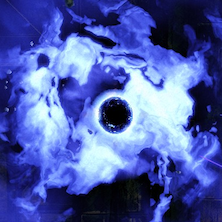
\includegraphics[scale=0.5]{pics/singularity.png}
	\caption{Logo projektu Singularity.}
	\label{singularity_logo}
\end{figure}

Do głównych cech rozwiązania istotnych z punktu widzenia administratora centrum danych są \cite{ad42}:
\begin{itemize}
\item Wsparcie dla konteneryzacji z wykorzystaniem technologi Docker lub konteneryzacji Mesos
\item Udostępnie zarówno interfejsu REST API jak i interfejsu graficznego w przeglądarce. 
\item Usługa równoważnenia obiążenia jest dostarczana przez firmę HubSpot w oddzielnym produkcie - Baragon.
\item Wsparcie dla sprawdzania zdrowia zadań (ang. \textit{Health Checks}) oraz wycofywania wysłanych transakcji.
\item Notyfikacje mailowe dotyczące zdarzeń na klastrze.
\item Możliwość generowania raportów dotyczących zdarzeń na klastrze.
\item Twórcy aplikacji pozostawili możliwość zaimplementowania własnych modułów, co umożliwia między innymi możliwość zaprojektowania własnego egzekutora dla zadań. 
\end{itemize}

Poniżej przedstawiono krótki plik w formacie JSON, który umożliwia uruchomienie kontenera Dockerowego używając obrazu hubspot/singularity-test-service:1.0, otwierając w nim dwa porty (8081, 8080) oraz rejestrują usługę sprawdzania zdrowia zadania na endpoincie /healthcheck. Zadanie będzie zużywać jeden procesor klastra i zarezerwuje 128 mega bajtów pamięci RAM.

\lstinputlisting[language=Json]{listings/singularity_example.json}

\subsection{Aurora}
Aurora (tab. \ref{aurora_info}, rys. (\ref{aurora_logo}) jest projektem rozwijanym przez fundację Apache w dużej części przez tych samych inżynierów co Mesos. Jego głównym wyróżnikiem jest sposób rezerwowania zasobów. Gdy większość frameworków działa na zasadzie otrzymania zadania do wykonania, a następnie próbie uzyskania zasobów do wykonania tego zadania, Aurora realizuje odwrotną politykę. Tuż po uruchomieniu Aurory, wszystkie zasoby klastra zostają przejęte przez framework, co powoduje szybsze uruchamianie zleconych zadań.

\begin{table}[!h]
\caption{Podsumowanie systemu szeregowania Aurora.}
\label{aurora_info}
\centering
\begin{tabular}{|p{4cm}|p{6cm}|}
  \hline
  \textbf{Język programowania} & Java, Python \\
  \hline
  \textbf{Licencja} & Wolne oprogramowanie, Apache 2.0. \\
  \hline
  \textbf{Tryb HA} & Brak. Musi zostać zapewniony innymi narzędziami. \\
  \hline
  \textbf{Firma rozwijająca} & Apache Fundation \\
  \hline
  \textbf{HTTP API} & Brak. \\
  \hline
  \textbf{UI} & TAK, ale bez możliwości urchamiania nowych zadań. \\
  \hline
\end{tabular}
\end{table}

\begin{figure}[!h]
	\centering
	
\includegraphics[scale=1]{pics/aurora_logo.png}
	\caption{Logo projektu Aurora.}
	\label{aurora_logo}
\end{figure}

Szczególnymi wyróżnikami projektu Aurora, są \cite{ad41}:
\begin{itemize}
\item Wsparcie dla konteneryzacji z wykorzystaniem technologi Docker lub konteneryzacji Mesos.
\item Dyrektywy dla \textit{scheduler'a} - możliwość określenia komputerów na których dane zadanie może być uruchomione wraz ze wskazaniem ile maksymalnie instancji może być jednocześnie uruchomionych.
\item Wsparcie dla planowania zadań (ang. \textit{cron jobs}.
\item Podobnie jak w mechaniźmie Singularity pozostawiono użytkownikowi zaimplementowanie własnych egzekutorów.
\item Uruchomienie zadania wymusza przygotowanie programu w języku Python. Umożliwia to doimplementowanie innych mechanizmów, które mogą się wykonywać wraz z zadaniem.
\end{itemize}

Jak widać w tabeli \ref{aurora_info} Aurora nie udostępnia API HTTP. Aby uruchomić zadanie w Aurorze należy przygotować dwa programy w języku Python. Pierwszy z nich będzie poleceniem do wykonania, zaś drugi będzie opisywał sposób uruchomienia zadania.

Kod prostego zadania, który będzie wypisywał linię a następnie zasypiał na zadany czas:
\lstinputlisting[language=Json]{listings/aurora_task.py}

Następnie należy przygotować program, który zdefinuje w jaki sposób podane zadanie ma być uruchomione:
\lstinputlisting[language=Json]{listings/aurora_run.py}

Aby uruchomić zadanie należy wykonać poniższe polecenie, jako parametr wskazując powyższy plik.
\begin{lstlisting}
aurora job create [klaster] [zadanie]
\end{lstlisting}

\newgeometry{top=2.5cm, bottom=2.5cm, left=2.5cm, right=3.5cm}
\onehalfspacing
\chapter{Praktyczna analiza przedstawionych rozwiązań}
\section{Przygotowania klastra do wykonania analizy}
\subsection{Specyfikacja techniczna klastra}
Na potrzeby przeprowadzenia pomiarów do niniejszej pracy magisterskiej otrzymałem poprzez mojego promotora sześć komputerów (rys. \ref{klaster_magisterski_photo}). Na każdym z nich zainstalowałem system operacyjny Ubuntu 16.04 oraz podstawowe aplikacje (openssh, serwer VPN etc). Do zarządzania klastrem (instalowanie paczek, ponowne uruchamianie itp) wykorzystałem nowoczesne rozwiązanie Ansible. Dostarczone komputery były identyczne, a każdy z nich posiada:
\begin{itemize}
\item Procesor Intel Core 2 Duo (E7400 @ 2x 2.80GHz)
\item 3GB pamięci RAM
\item Dysk twardy o rozmiarze 500GB
\end{itemize}

Jeden z komputerów nie został włączony do klastra i posłużył jako host do zarządzania pozostałymi komputerami. Pozostałe 5 komputerów posłużyło do instalacji klastra. Na każdym z nich został zainstalowany Docker, Mesos oraz Kubernetes. Jeden z komputerów posłużył jako master, zaś pozostałe 4 zostałe wykorzystane jako komputery agenty. W tabeli \ref{klaster_magisterski} przedstawiono konfigurację klastra.

\begin{table}[!h]
\caption{Role poszczególnych komputerów w klastrze.}
\label{klaster_magisterski}
\centering
\begin{tabular}{|p{2cm}|p{2cm}|p{2cm}|p{2cm}|p{2cm}|p{2cm}|p{2cm}|}
  \hline
   & 192.168.0.11 & 192.168.0.12 & 192.168.0.13 & 192.168.0.14 & 192.168.0.15 & 192.168.0.16 \\
  \hline
  \textbf{Rola} & Zarządzanie & Kontroler & Node & Node & Node & Node \\
  \hline
  \textbf{Docker} & TAK & TAK & TAK & TAK & TAK & TAK \\
  \hline
  \textbf{Rkt} & TAK & NIE & NIE & NIE & NIE & NIE \\
  \hline
  \textbf{Kubernetes} & NIE & Master & Worker & Worker & Worker & Worker \\
  \hline
  \textbf{Mesos} & NIE & Master & Agent & Agent & Agent & Agent \\
  \hline
\end{tabular}
\end{table}

\begin{figure}[!h]
	\centering
	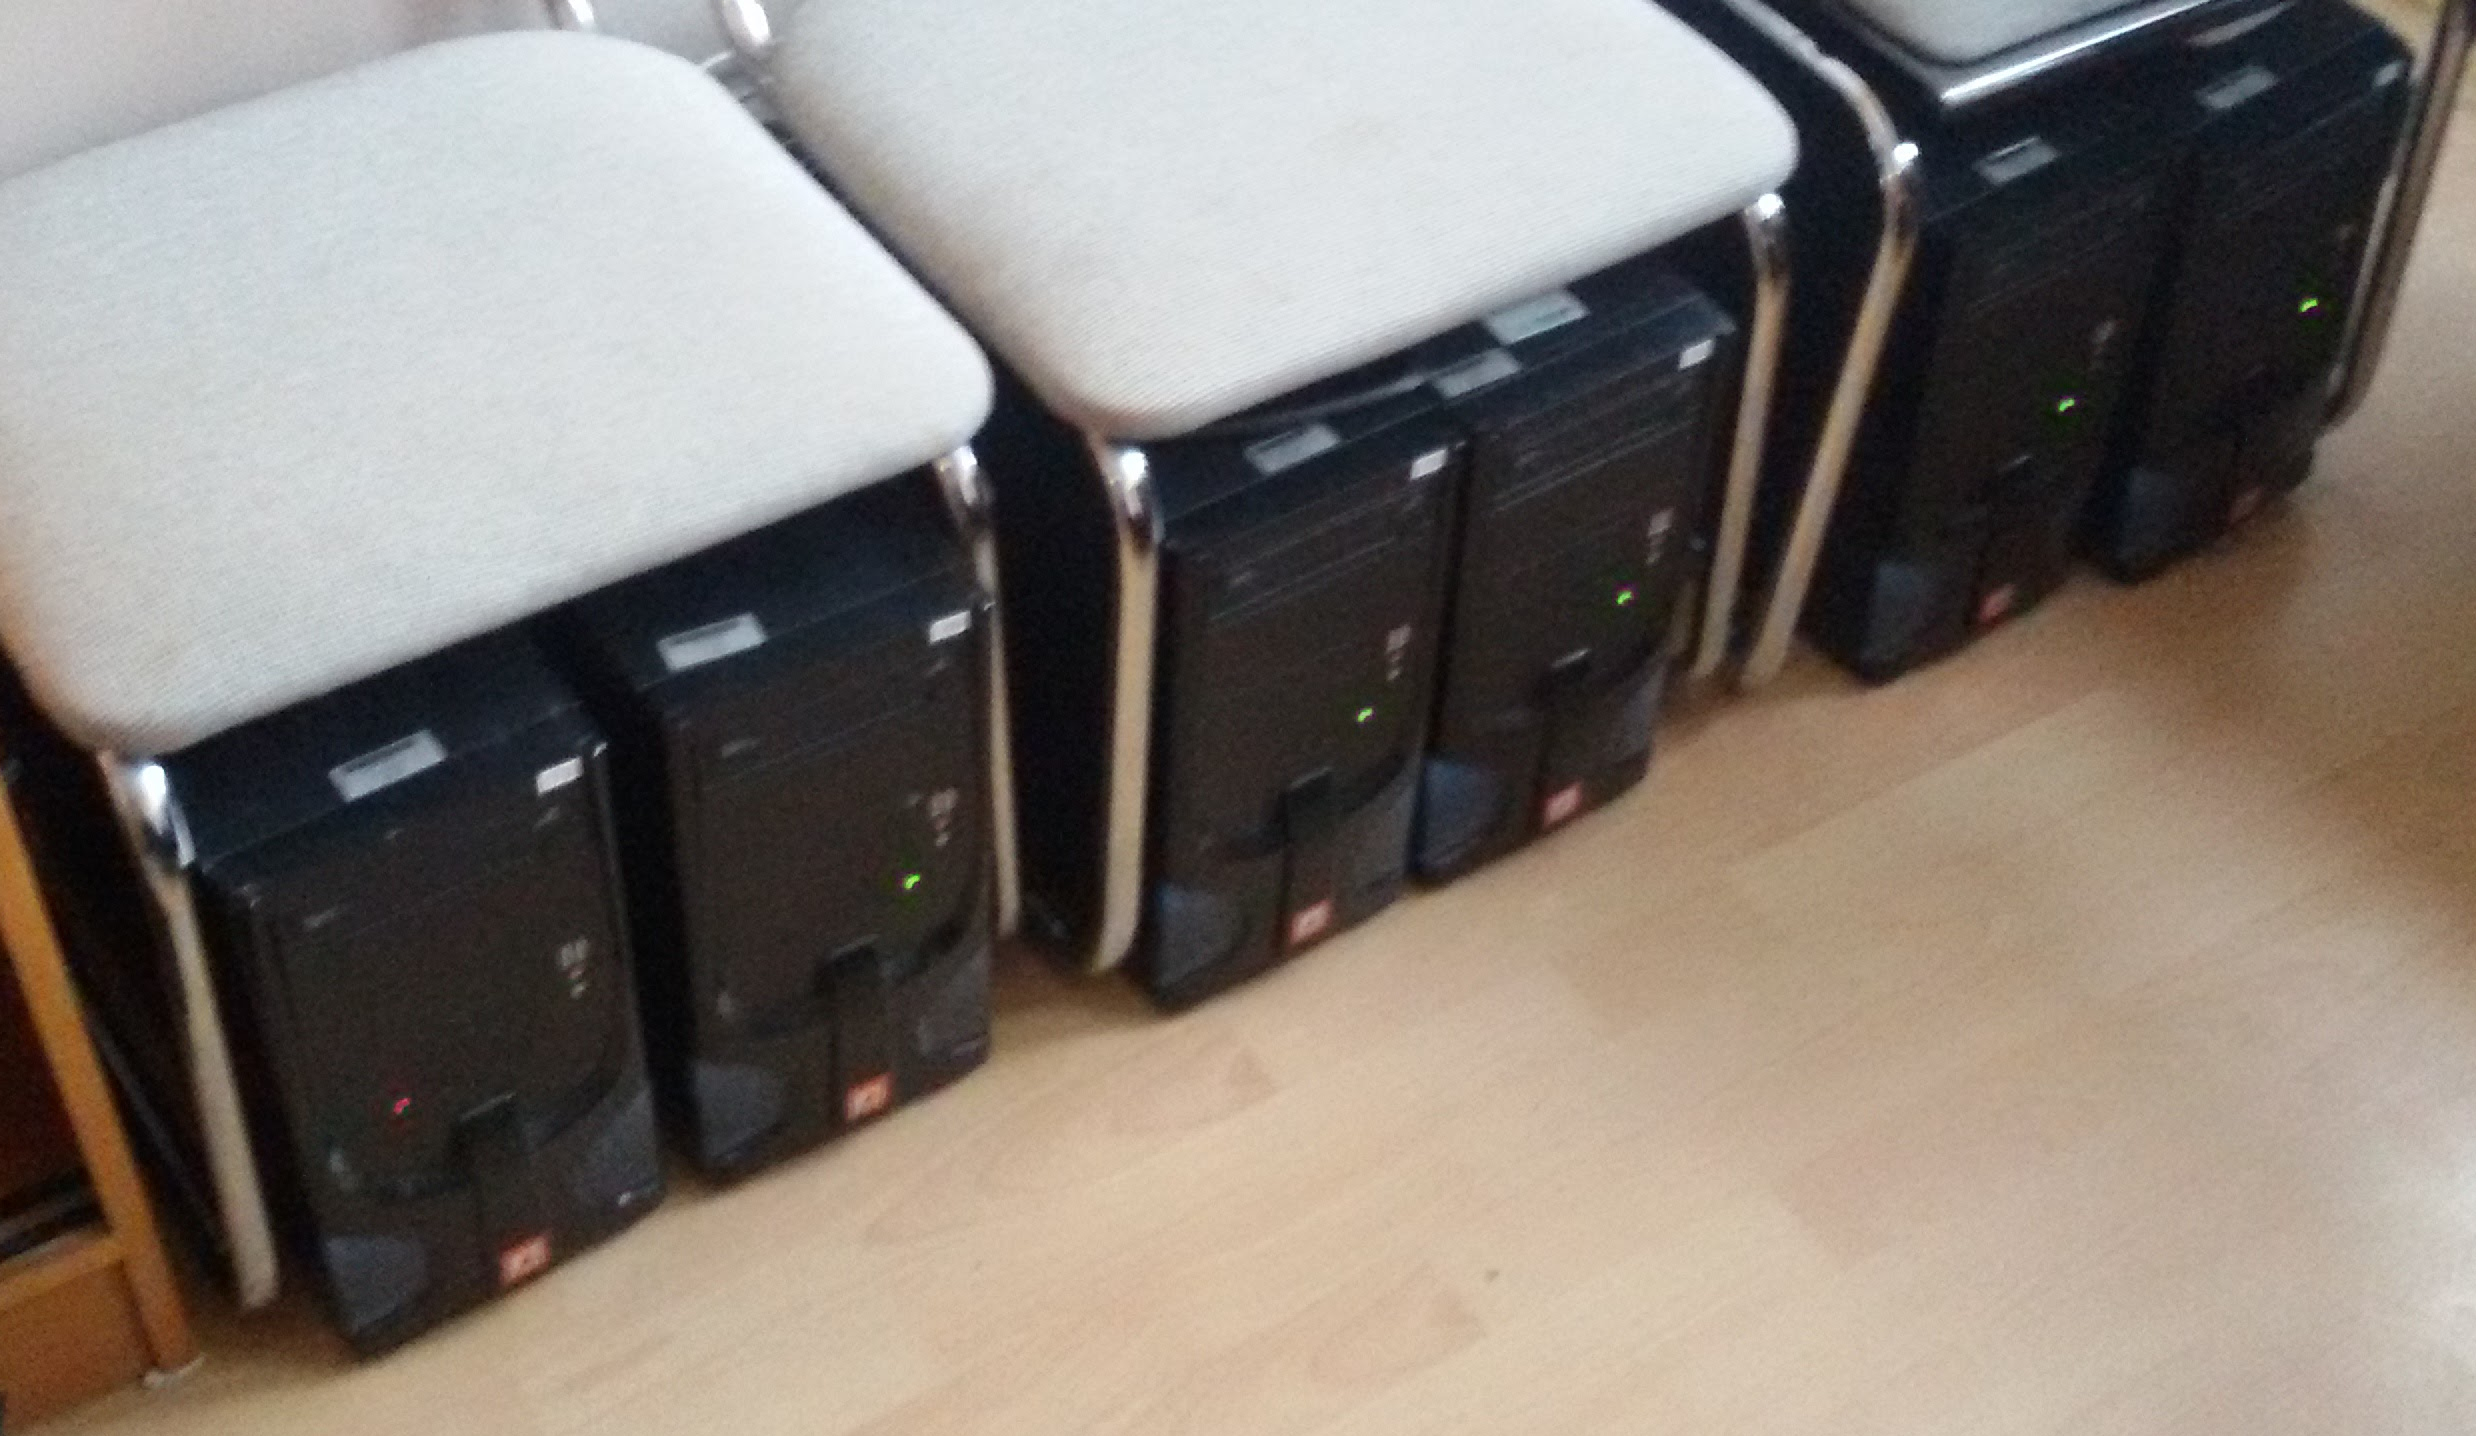
\includegraphics[scale=0.15]{pics/20170308_163141.jpg}
	\caption{Komputery użyte do wykonania badań.}
	\label{klaster_magisterski_photo}
\end{figure}

W ten sposób udało się uzyskać następującą ilość zasobów, które mogły by rezerwowane przez Mesos'a do wykonywania zadań:
\begin{itemize}
\item 8 procesorów o taktowaniu 2.80GHz każdy,
\item 12GB pamięci RAM,
\item Pamięć dyskową o powierzchni prawie 4TB.
\end{itemize}

\subsection{Sposób instalacji Mesos'a na klastrze}
Aby zainstalować oprogramowanie Mesos na potrzeby tej pracy przygotowałem własne obrazy dla aplikacji mesos-master oraz mesos-slave. Ich kod został opublikowany w serwisie github.com a zbudowane obrazy zostały opublikowane w serwisie quay.io oraz dockerhub. Aby pobrać stworzony przeze mnie obraz oprogramowaniem docker należy wykonać polecenie:
\begin{lstlisting}
docker pull quay.io/mesosdockerized/mesos-master
docker pull quay.io/mesosdockerized/mesos-slave
\end{lstlisting}

Zaś kod obu obrazów dostępny jest tutaj:
\begin{lstlisting}
https://github.com/mesos-dockerized/master-dockerfile
https://github.com/mesos-dockerized/slave-dockerfile
\end{lstlisting}

Usługi mesos-master i mesos-slave kontrolowane są przez odpowiednie pliki konfiguracyjne \textit{systemd}. Odpowiednio dla mastera:
\lstinputlisting[language=Json]{listings/mesos-master.service}

Dla agenta:
\lstinputlisting[language=Json]{listings/mesos-slave.service}

Dla usług uruchamianych w kontenerach konieczne było zastsowanie kilku dodatkowych flag:
\begin{itemize}
\item MESOS\_NO\_HOSTNAME\_LOOKUP - Ze względu na brak serwera DNS na klastrze, ustawienie tej zmiennej jest konieczne by Mesos nie próbował rozwiązywać nazwy pozostałych serwisów. 
\item MESOS\_REGISTRY - Uruchomienie procesu mastera w kontenerze powoduje, że po jego zakończeniu wszelkie logi znikną razem z kontenerem. Esportując jednocześnie flagę MESOS\_WORK\_DIR i MESOS\_LOG\_DIR wymuszamy zapis logów i informacji roboczych na dysku gospodarza. W ten sposób nawet po restarcie kontenera stan klastra jest zachowany.
\item MESOS\_SYSTEMD\_ENABLE\_SUPPORT - Nie jest możliwe uruchomienie uruchomienie Mesosa ze wsparciem \textit{systemd}, ponieważ \textit{systemd} nie jest używane wewnątrz kontenera.
\end{itemize}
Kluczowym w uruchomieniu procesu mesos-slave w kontenerze jest przekazanie do jego wnętrza części plików gospodarza. Są to zarówno \textit{control-groupy} z systemu gospodarza oraz zainstalowana aplikacja dockera. Ten zabieg jest niezbędny by zadania Mesosa, które mają być uruchamiane w Dokerze, uruchomiły się w systemie operacyjnym gospodarza.

Obrazy Zookeepera, Marathona i Singularity zostały pobrane z internetu a ich konfiguracja znajduje się poniżej. Framework Aurora, został zainstalowany "klasycznie", gdyż ze względu na jego poziom skomplikowania i architekturę, bardzo trudne jest jego umieszczenie w kontenerze. 

Konfiguracja kontenera z Zookeeperem:
\lstinputlisting[language=Json]{listings/zookeeper.service}

Konfiguracja kontenera z frameworkiem Marathon:
\lstinputlisting[language=Json]{listings/marathon.service}

Konfiguracja kontenera z frameworkiem Singularity:
\lstinputlisting[language=Json]{listings/singularity.service}

\section{Przeprowadzone pomiary i analizy}
Po przeprowadzeniu i udokumentowaniu procesu instalacji dokonałem pomiarów związanych z czasem startu zadań uruchamianych przez poszczególne frameworki. Dodatkowo dokonałem prostego sprawdzenia testów izolacji we wcześniej opisanych rozwiązaniach.

\subsection{Czas uruchomienia zadań}
Do testu został wybrany bardzo popularny obraz \textit{httpd}. Obraz należy do grupy obrazów wspieranych oficjalnie przez firmę Docker. 
\begin{lstlisting}
https://hub.docker.com/_/httpd/
\end{lstlisting}

Obraz może być pobrany poleceniem:
\begin{lstlisting}
docker pull httpd
\end{lstlisting}

Test polega na pobraniu aktualnej godziny z systemu operacyjnego a następnie wysłanie do frameworka polecenia uruchamiającego zadanie opierające się o podany wyżej obraz. Kontener z obrazem httpd wystawi serwer http na porcie 80. Test będzie oczekiwał na otwarcie tego portu, a gdy to się wydarzy ponownie pobierze czas z systemu operacyjnego i odejmie go od tego pobranego na początku. W ten sposób uzyskam informację ile czasu trwało uruchomienie zadania. Tak przygotowany test został uruchomiony 10 tysięcy razy dla każdego frameworka a uśredniony wynik został przedstawiony w tabeli \ref{framework_results}. Poniżej przedstawiam kod potrzebny do wykonania pojedyńczego pomiaru dla frameworka Marathon.

Definicja zadania (task.json):
\lstinputlisting[language=Json]{listings/test_job.json}

Uruchomienie podanej powyżej definicji i oczekiwanie na jego uruchomienie można zrealizować poniższym skryptem (tester.sh):
\lstinputlisting[language=Json]{listings/tester.sh}

Pojedyńczy pomiar można dokonać mierząc czas wykonania skryptu za pomocą polecenia time.
\begin{lstlisting}
time ./tester.sh
\end{lstlisting}

\begin{table}[!h]
\caption{Uśrednione wyniki czasu uruchamiania zadań na poszczególnych frameworkach.}
\label{framework_results}
\centering
\begin{tabular}{|p{4cm}|p{4cm}|}
  \hline
  \textbf{Framework} & \textbf{Uśredniony czas [s]} \\
  \hline
  Marathon & 1.117s \\
  \hline
  Singularity & 1.267s \\
  \hline
  Aurora & 0.870s \\
  \hline
\end{tabular}
\end{table}

\subsection{Testy izolacji}
Testy izolacji polegały na uruchomieniu w różnych rozwiązaniach i konfiguracjach obrazu kontenerowego z zaszytą w środku fork-bombą. Fork bomba jest to implementacja nieskończonej pętli w której uruchamia się kolejna instancja tego samego procesu. Atak opiera się na bardzo szybkim rezerwowaniu zasobów pod kolejne procesy oraz na rezerwowaniu czasu procesora na wykonanie każdego nowo stworzonego procesu. Fork-bomba jest skrajnym i bardzo trudnym do wyizolowania przypadkiem. Celem moich testów było stwierdzenie w jakim stopniu poszczególne przedstawione rozwiązania radzą sobie z takim przypadkiem. Za pełny sukces uznam sytuację w której uruchomiony kontener z forkbombą nie będzie wpływał na uruchomiony system oraz inne uruchomione kontenery.

Do przeprowadzenia testu został wykorzystany obraz oparty o następujący plik \textit{Dockerfile}:
\lstinputlisting[language=Json]{listings/Dockerfile}

Poniżej przedstawiam rezultat uruchomienia powyższego obrazu w poszczeglnych konfiguracjach:
\begin{itemize}
\item Konteneryzacja Dockera - po uruchomieniu obrazu poleceniem docker run i pozostawieniu systemu operacyjnego na 30 minut została dokonana analiza. Docker jako aplikacja klient serwer przestała być użyteczna. Nie było możliwe wykonanie żadnego polecenia poprzedzonego słowem 'docker'. Z tego względu nie było możliwe uruchomienie żadnego nowego kontenera, ani wejście do już istniejącego. Jednakże inny kontener uruchomiony na tym samym komputerze (httpd) odpowiadał na żądania na porcie 80. System operacyjny był stabilny, ale dało się odczuć zaczący spadek responsywności systemu. Wykonując niektóre polecenia system zwracał informacje o braku pamięci.
\item Konteneryzacja rkt z mechanizmem \textit{fly} - zgodnie z oczekiwaniem uruchomienie kontenera miało wpływ na system operacyjny. Pamięć rezerwowana przez proces kontenera była jednocześnie pamięcią, którą mógł rezerwować system operacyjnym. W ciągu kilku minut system przestał być stabilny, przestało działać SSH a jedynym sposobem na odzyskanie stabilności był restart systemu.
\item Konteneryzacja rkt w oparciu o c-grupy - doszło do bardzo podobnego zachowania jak przy konteneryzacji aplikacją Docker. Widoczny był spadek responsywności systemu natomiast możliwe było uruchamianie nowych kontenerów.
\item Konteneryzacja rkt z mechanizmem \textit{qemu/lkvm} - zgodnie z oczekiwaniem proces nie był w stanie przejąć pamięci systemu operacyjnego, poza tą przejętą przez maszynę wirtualną.
\item Mesos z konteneryzacją Docker'a - Mesos nie dostarcza żadnego dodatkowego mechanizmu izolacji poza uruchomieniem kontenera Dockera. Dlatego system zachowuje się identycznie jak przy uruchomieniu pojedyńczego kontenera dockerowego.
\item Mesos z wykorzystaniem konteneryzacji natywnej - system operacyjny został zdławiony brakiem pamięci (podobnie jak przy \textit{rkt-fly}). Jedynym sposobem by odzyskać sprawność systemu był jego restart. Niestety po utracie kontaktu z agentem, Mesos uruchomił problematyczne zadanie na innym komputerze, również destabilizując go.
\item Kubernetes - przy domyślnej konfiguracji zadanie zostanie uruchomione w kontenerze Dockerowym i system zostanie doprowadzony do stanu jak z pierwszego punktu. Jednakże kubernetes posiada możliwość uruchomienia zadania z narzuconymi limitami. Wykorzystując ten mechanizm udało się odizolować zadanie od systemu operacyjnego. 
\end{itemize}

\newgeometry{top=2.5cm, bottom=2.5cm, left=2.5cm, right=3.5cm}
\onehalfspacing
\chapter{Podsumowanie wykonanej analizy}
Opierając się na testach analizy izolacji oraz czasu uruchamiania, można stwierdzić, że najbardziej uniwersalnym rozwiązaniem jest wykorzystanie Mesosa z systemem szeregowania Marathon i uruchamianie zadań w oparciu o system konteneryzacji Docker. Jednakże w bardziej specyficznych przypadkach: 
\begin{itemize}
\item Wiele pojedyńczych zadań obliczeniowych - gdy najważniejszym kryterium jest szybkie uruchamianie zadań najbardziej efektywnym systemem szeregowania wydaje się być Aurora. Decydującą przewagą jest tutaj rezerwowanie wszytkich zasobów klastra, dzięki czemu framework omija fazę negocjowania ofert z zasobami. Jedncześnie powoduje to, że nie jest możliwe zainstalowanie żadnego innego frameworka na klastrze. Innym problemem związanym z wykorzystaniem tego frameworka, jest poziom skomplikowania w kwesti uruchamiania zadań, natomiast w przypadku bardzo częstego uruchamiania zadań warto zainwestować w implementację tego mechanizmu.
\item Niewielka ilość zadań obliczeniowych - system szeregowania Singularity posiada typ zadań \textit{One-shoot}. Umożliwia on wykonanie pojedyńczej pracy bez ponownego uruchamiania procesu po jego zakończeniu. Jeśli czas startu nie jest priorytetem to użycie frameworka Singularity pozwoli na uruchamianie zadań obliczeniowych bez żadnych dodatkowych implementacji, pozwalając jednocześnie na używanie innych systemów szeregowania. 
\item Zadania typu serwis - jeśli celem klastra jest serwowanie treści i równoważenie obciążenia to zarówno system szeregowania Marathon jak i Singularity wydają się spełniać oczekiwania. W systemie Singularity przygotowane jest rozwiązanie do równoważenia obciążenia, natomiast przy wykorzystaniu frameworka Marathon należy zatroszyć się o to rozwiązanie samemu (bazując na przykład na zananym rozwiązaniu - HAProxy).
\item Zadania w których izolacja jest najważniejsza - gdy kontener ma zostać udostępniony bezpośrednio klientowi końcowemu lub też aplikacja działająca w kontenerze jest niestabilna jeśli chodzi o wykorzystanie zasobów, najbezpieczniej jest wykorzystać rozwiązanie rkt wraz z obsługą KVM'a (qemu lub lkvm). Wsparcie dla tych rozwiązań posiada orkiestrator Kubernetes.
\end{itemize}

Analiza obecnych rozwiązań wskazuje kilka problemów, które mogłby być miejscem do dalszych prac inżynierskich:
\begin{itemize}
\item System konteneryzacji Docker powinien radzić sobie z izolowaiem fork bomby bez żadnych dodatkowych konfiguracji i parametrów.
\item Orkiestrator Mesos powinienn wspierać różne mechanizmy konteneryzacji. Aktualnie nie jest możliwe użycie Mesosa z rozwiązaniem rkt.
\item Orkiestrator Mesos powinien oferować mechanizm który uruchomi kontener w taki sposób by jego izolowanie było skuteczne. Taki mechanizm zaimplementowany jest w Kubernetesie (\textit{limits}).
\item System konteneryzacji rkt w swoim domyślnym rozwiązaniu konteneryzacyjnym powinien skutecznie izolować problemy typu fork bomby.
\end{itemize}

Wracają do pytania postawionego na samym początku tej pracy pytania, odpowiednie przygotowanie i skonfigurowanie klastra Mesos'a umożliwia zwiększenie poziomu utylizacji w centrum danych. Dla większości zastosowań obecne systemy izolacji powinny być wystarczające, zaś mechanizm etykiet, które udostępniają \textit{frameworki} pozwoli na odpowiedzialne rozdzielenie zadań pomiędzy fizyczne serwery w DC. W pracy przedstawiłem również alternetywne rozwiązania, które mogą znaleźć zasotosowanie w sytuacjach w których Mesos nie będzie wystarczający.

\listoffigures
\addcontentsline{toc}{chapter}{Spis rysunków}

\newpage

\listoftables
\addcontentsline{toc}{chapter}{Spis tabel}


\begin{thebibliography}{99}
\bibitem{ad1}Hamilton J., \textit{Internet-Scale Service Infrastructure Efficiency}, Symposium on Computer architecture, Jun. 2009.
\bibitem{ad2}Linthicum D., \textit{How to integrate with the cloud}, InfoWorld: Cloud Computing, April 27, 2011.
\bibitem{ad3}Kozyrakis Ch., \textit{Resource Efficient Computing for Warehouse-scale Datacenters}, 2013, Stanford University.
\bibitem{ad4}Carlson N., \textit{At Last — The Full Story Of How Facebook Was Founded}, Business Insider.
\bibitem{ad5}Data Center Knowledge blog [online].[dostęp 26.03.2017]. Dostępny w Internecie: http://www.datacenterknowledge.com/the-facebook-data-center-faq/
\bibitem{ad6}"Chip",\textit{Internet jest chmurą}, 03/2009, s. 38. Warszawa: Burda Communications sp. z o.o.. ISSN 1230-817X.
\bibitem{ad7}Trojnar D.,\textit{Wirtualizacja jako przyszłość sieci teleinformatycznych}, W: SECON 2010 – Materiały konferencyjne. Warszawa: WAT, 2010.
\bibitem{ad8}Levinson M., \textit{Software as a Service (SaaS) Definition and Solutions}.
\bibitem{ad9}Boniface, M., \textit{Platform-as-a-Service Architecture for Real-Time Quality of Service Management in Clouds}, 5th International Conference on Internet and Web Applications and Services (ICIW), Barcelona, Spain: IEEE, pp. 155–160, doi:10.1109/ICIW.2010.91
\bibitem{ad10}Mell P., Grence T., \textit{The NIST Definition of Cloud Computing (Technical report)}, MNational Institute of Standards and Technology: U.S. Department of Commerce. doi:10.6028/NIST.SP.800-145. Special publication 800-145.
\bibitem{ad11}Rouse M.,\textit{What is public cloud?}, Definition from Whatis.com.
\bibitem{ad12}Bernstein D., Ludvigson E., Sankar K., Diamond S., Morrow M., \textit{Blueprint for the Intercloud – Protocols and Formats for Cloud Computing Interoperability}, IEEE Computer Society: 328–336. doi:10.1109/ICIW.2009.55. ISBN 978-1-4244-3851-8.
\bibitem{ad13}Krause S.,\textit{The private vs public cloud debate: Which to deploy, and why consider hybrid?}, cloudcomputing news.
\bibitem{ad14}Freedman R., \textit{Cloud computing migration issues: What you need to know} [online].[dostęp 14.04.2017]. Dostępny w Internecie: http://www.techrepublic.com/blog/it-consultant/cloud-computing-migration-issues-what-you-need-to-know/.
\bibitem{ad15}Krasuski T., Łoś J., Szostakiewicz M.,\textit{Wstęp do wirtualizacji}, Uniwersytet Warszawski, 2005. 
\bibitem{ad16}Mesos Community, \textit{Powerd By Mesos, Organizations using Mesos}, http://mesos.apache.org/documentation/latest/powered-by-mesos/ (data dostępu: 14.04.2017).
\bibitem{ad17}Anton Beloglazov, Rajkumar Buyya, \textit{Energy Efficient Resource Management in Virtualized Cloud Data Centers}, The University of Melbourne, Australia, 2010.
\bibitem{ad18}Gabriel Cephas Obasuyi, Arif Sari, \textit{Security Challenges of Virtualization Hypervisors in Virtualized Hardware Environment}, SciRes, 2015.
\bibitem{ad19}James F. Brady, \textit{Virtualization and CPU wait times in a Linux guest environment}, Capacity Planner for the State Of Nevada.
\bibitem{ad20}Ronald L. Krutz, Russell Dean Vines, \textit{Cloud Security: A Comprehensive Guide to Secure Cloud Computing}, Wiley Publishing, 2010, ISBN:0470589876
\bibitem{ad21}Wes Felter, Alexandre Ferreira, Ram Rajamony, \textit{An updated performance comparison of virtual machines and Linux containers}, IBM Research Department, Austin, Texas
\bibitem{ad22}A. Avram, \textit{Docker: Automated and Consistent Software Deployments}, 2013, infoq.com
\bibitem{ad23}Appc community, \textit{Docker: Appc spec}, https://github.com/appc/spec, (data dostępu 14.04.2017)
\bibitem{ad24}Docker community, \textit{Docker best practices}, https://docs.docker.com/engine/userguide/eng-image/dockerfile\_best-practices/\#general-guidelines-and-recommendations, (data dostępu 14.04.2017)
\bibitem{ad25}Thehftguy, \textit{Docker in production an history of failure}, https://thehftguy.com/2016/11/01/docker-in-production-an-history-of-failure, (data dostępu 14.04.2017)
\bibitem{ad26}Ewing Lusk, William Gropp, \textit{A high-performance, portable implementation of the MPI message passing interface standard}, The University of Utah
\bibitem{ad27}Sébastien Goasguen, \textit{Docker Cookbook}, 2015, O'Reilly Media
\bibitem{ad28}Bilal Sheikh, \textit{Comparing four hosted docker registries}, http://rancher.com/comparing-four-hosted-docker-registries/, (data dostępu 16.04.2017)
\bibitem{ad29}Rkt community, \textit{rkt code repository}, https://github.com/rkt/rkt, (data dostępu 20.04.2017)
\bibitem{ad30}Rkt community, \textit{rkt stages}, https://github.com/rkt/rkt/blob/master/Documentation/devel/architecture.md, (data dostępu 21.04.2017)
\bibitem{ad31}Rkt community, \textit{Introduce QEMU support}, https://github.com/rkt/rkt/pull/2952, (data dostępu 4.05.2017)
\bibitem{ad32}Rkt community, \textit{Rkt monitor results of start/stop time with different flavors}, https://github.com/rkt/rkt/issues/3019\#issuecomment-246637570, (data dostępu 4.05.2017)
\bibitem{ad33}Benjamin Hindman, Andy Konwinski, Matei Zaharia, Ali Ghodsi, Anthony D. Joseph, Randy Katz, Scott Shenker, Ion Stoica, \textit{Mesos: A Platform for Fine-Grained Resource Sharing in the Data Center}, University of California, Berkeley.
\bibitem{ad34}Roger Ignazio \textit{Mesos in Action}, 2016, ISBN: 9781617292927 
\bibitem{ad35}Marko Lukša \textit{Kubernetes in Action}, 2016, ISBN: 9781617293726
\bibitem{ad36}Hitachi Data Systems, \textit{Kubernetes on Hitachi Unified Compute Platform}, https://www.hds.com/en-us/pdf/white-paper/kubernetes-on-hitachi-ucp-whitepaper.pdf, (data dostępu 15.05.2017)
\bibitem{ad37}Rimantas Mocevicius \textit{CoreOS Essentials}, 2015, ISBN: 9781785283949
\bibitem{ad38}Mesos community, \textit{Mesos HTTP Endpoints}, http://mesos.apache.org/documentation/latest/endpoints/, (data dostępu 2.06.2017)
\bibitem{ad39}Mesos community, \textit{Mesos Observability Metrics}, http://mesos.apache.org/documentation/latest/monitoring/, (data dostępu 22.06.2017)
\bibitem{ad40}Mesos community, \textit{Mesos Modules}, http://mesos.apache.org/documentation/latest/modules/, (data dostępu 22.06.2017)
\bibitem{ad41}Dharmesh Kakadia, \textit{Apache Mesos Essentials}, 2015, ISBN: 1783288760
\bibitem{ad42}Mesosphere, \textit{Dawn of the Singularity: A look at HubSpot’s first year on Mesos}, https://mesosphere.com/blog/dawn-of-the-singularity-a-look-at-hubspots-first-year-on-mesos/, (data dostępu 30.07.2017)
\bibitem{ad43}Wojciech Tyczyński, \textit{Scalability updates in Kubernetes 1.6: 5,000 node and 150,000 pod clusters}, http://blog.kubernetes.io/2017/03/scalability-updates-in-kubernetes-1.6.html, (data dostępu 15.09.2017)
\bibitem{ad44}Adam Bordelon Niklas, Quarfot Nielsen, \textit{Mesos, Elastically Scalable Operations, Simplified}, http://mesosphere.github.io/presentations/oscon-mesos-ops-2014/full/, (data dostępu 15.09.2017)
\end{thebibliography}

\addcontentsline{toc}{chapter}{Bibliografia}

\end{document}
